\documentclass{homework}

\title{I2}
\date{2020-06-9}
\gdate{1er Semestre 2020}
\author{Nicholas Mc-Donnell}
\course{Geometría Diferencial - MAT2305}

\setkeys{Gin}{width=.9\textwidth}

\begin{document}
\maketitle
\newpage
\pagenumbering{arabic}

\begin{sol}
    \begin{enumerate}
        \item Sea \(S_2\) una superficie regular orientable, y sea \(S_1\subset S_2\) una superficie regular. Ahora, sea \(N\) la orientación de \(S_2\), y \(N'\) la restricción de \(N\) a \(S_1\). Si \(N'\) no es una orientación de \(S_1\), entonces existe algún punto \(p\in S_1\) donde \(N'\) no está bien definida, como \(p\in S_1\), se tiene que \(p\in S_2\), más aún como \(\forall q\in S_1 N(q)=N'(q)\) \(N\) no está bien definida en \(p\in S_2\), pero eso es una contradicción ya que \(N\) es una orientación de \(S_2\). Por lo que \(S_1\) es orientable.
        \item Sean \(S_1, S_2\) superficies regulares difeomorfas, además \(S_1\) es orientable. Sea \(\varphi:S_1\rightarrow S_2\) un difeomorfismo, luego \(\d{\varphi}:TS_p(S_1)\rightarrow TS_p(S_2)\) es un isomorfismo. Sea \(p\in S_1\) un punto, ahora sean \(\hat{\vec{x}}_u,\hat{\vec{x}}_v\) los vectores correspondientes normalizados. Se define \(N'=\frac{\d{\varphi}\hat{\vec{x}}_u\wedge\d{\varphi}\hat{\vec{x}}_v}{\det(\d{\varphi})}\), \(N'\) está bien definida
        \item Sea \(S\) una superficie regular tal que la Banda de Möbius es un subconjunto de ella, se asume que \(S\) es orientable, por (a) el subconjunto que corresponde a la Banda de Möbius es orientable, pero hay un difeomorfismo natural de ese subconjunto a la Banda de Möbius misma, y por (b) se tendría que la Banda de Möbius es orientable, lo que es una contradicción. Por ende \(S\) no es orientable.
    \end{enumerate}
\end{sol}

\begin{sol}
    \begin{enumerate}
        \item Usando que \(\vec{x}_u=(\cos v,\sin v,2u\sin v)\) y que \(\vec{x}_v=(-u\sin v,u\cos v,u^2\cos v)\) se llega lo siguiente\footnote{Los cálculos están en el apendice.}:
        \begin{align*}
            E&=4u^2\sin^2v+1\\
            F&=2u^3\sin v\cos v\\
            G&=u^2+u^4\cos^2 v
        \end{align*}
        \item Usando que \(\vec{x}_{uu}=(0,0,2\sin v)\), \(\vec{x}_{uv}=(-\sin v,\cos v, 2u\cos v)\), \(\vec{x}_{vv}=(-u\cos v,-u\sin v,-u^2\sin v)\), y que \(N=\frac{(u\sin v\cos v,-u(1+\sin^2 v),1)}{\sqrt{u^2(3\sin^2v+1)+1}}\) se llega\footnote{Ver 1.} a que:
        \begin{align*}
            e&=\frac{2\sin v}{\sqrt{u^2(3\sin^2v+1)+1}}\\
            f&=\frac{u^2\cos v}{\sqrt{u^2(3\sin^2v+1)+1}}\\
            e&=\frac{u^3\sin v}{\sqrt{u^2(3\sin^2v+1)+1}}\\
        \end{align*}
        \item Usando que \(K=\frac{eg-f^2}{EG-F^2}\) y los valores ya calculados se llega\footnote{Ver 1.} a que \(K=\frac{u(\sin^2v-u\cos^v)}{(u^2(3\sin^2v+1)+1)^2}\).
        \item Usando los coeficientes cálculados anteriormente, se cálcula la matriz de \(\d{N}_{(1,0)}\) en base \(\{\vec{x}_u,\vec{x}_v\}\):
        \begin{equation*}
            \d{N}_{(1,0)}=\begin{pmatrix}
                0 & -\frac1{\sqrt{2}}\\
                -\frac1{2\sqrt{2}} & 0\\
            \end{pmatrix}
        \end{equation*}
        Se calculan\footnote{Ver 1.} sus valores propios son \(k_1=\frac12,k_2=-\frac12\), y sus vectores propios son \(v_1=(-\sqrt{2},1),v_2=(\sqrt{2},1)\). Por definición \(k_1,k_2\) son las curvaturas principales y \(v_1,v_2\) las direcciones principales
    \end{enumerate}
\end{sol}

\begin{sol}
    \begin{enumerate}
        \item Usando que \(\vec{x}_r=(\cos\theta,1+\sin\theta,5)\) y que \(\vec{x}_\theta=(-r\sin\theta,r\cos\theta,0)\), se hacen unos cálculos\footnote{Ver 1.} y se llega a \(N=\frac{(-5\cos\theta,-5\sin\theta,1+\sin\theta)}{\sqrt{(1+\sin^2\theta)^2+25}}\), lo cual no depende de \(r\). Ahora, sea \(\alpha(r)=\vec{x}(r,\theta_1)=r(\cos\theta,1+\sin\theta,5)\), luego \(\alpha'(r)=(\cos\theta,1+\sin\theta,5)\) y \(N'(r)=\vec{0}=0\cdot\alpha'(r)\), por lo que por Olinde Rodrigues \(\alpha\) es linea de curvatura.
        \item Sea \(\alpha(\theta)=\vec{x}(r_1,\theta)\), se tiene que \(\alpha''(\theta)=(-r_1\cos\theta,-r_1\sin\theta,0)\). Luego, con \(n=\frac{\alpha''}{\norm{\alpha''}}\) se tiene que \(k_n=\frac{5r_1}{\sqrt{(1+\sin^2\theta)^2+25}}>0\). Ahora, como \(N\) no depende de \(r\), se tiene que \(\det(\d{N})=0\), por lo que \(K=0\), por lo que dado \(k_1\geq k_2\) y usando continuidad de \(k_n\) se tiene que \(k_2=0\), más aún como \(k_n>0\), para \(n=\frac{\alpha''}{\norm{\alpha''}}\), se tiene que \(k_1>0\). Este argumento funciona para todo punto en alguna curva \(\alpha_{r_1}\), y como todo punto está en alguna de estas curvas, se tiene que todo punto tiene que \(k_1>k_2=0\), por lo que todos los puntos son parabólicos.
        \item 
    \end{enumerate}
\end{sol}

\begin{sol}
    \begin{enumerate}
        \item Dado que \(\varphi_x=-2x\) y \(\varphi_y=2y\) se tiene que \(\vec{x}_x=(1,0,-2x)\) y que \(\vec{x}_y=(0,1,2y)\). Se usa esto para calcular \(E,F\) y \(G\)\footnote{Ver 1.}:
        \begin{align*}
            E&=4x^2+1\\
            F&=-4xy\\
            G&=4y^2+1
        \end{align*}
        Dado eso se calcula\footnote{Ver 1.} \(c=EG-F^2=4x^2+4y^2+1\), y se usa para calcular los símbolos de Christoffel\footnote{Ver 1.}:
        \begin{align*}
            \Gamma^1_{1 1}&=\frac{4x}{4x^2+4y^2+1}\\
            \Gamma^2_{1 1}&=\frac{-4y}{4x^2+4y^2+1}\\
            \Gamma^1_{1 2}&=0\\
            \Gamma^2_{1 2}&=0\\
            \Gamma^1_{2 2}&=\frac{-4x}{4x^2+4y^2+1}\\
            \Gamma^2_{2 2}&=\frac{4y}{4x^2+4y^2+1}
        \end{align*}
        \item Con los símbolos de Christoffel y la siguiente fórmula:
        \begin{equation*}
            K=-\frac1{E}\paren{(\Gamma^2_{1 2})_x-(\Gamma^2_{1 1})_y+\Gamma^1_{1 2}\cdot\Gamma^2_{1 1}-\Gamma^1_{1 1}\Gamma^2_{1 2}+\Gamma^2_{1 2}\Gamma^2_{1 2}-\Gamma^2_{1 1}\Gamma^2_{2 2}}
        \end{equation*}
        Después de unos cálculos\footnote{Ver 1.} se llega a:
        \begin{equation*}
            K=\frac{-4}{(4x^2+4y^2+1)^2}<0
        \end{equation*}
        Como \(K<0\) se tiene que el paraboloide no puede ser localmente isometrico al plano, ya que la curvatura Gaussiana es invariante a través de isometrías locales\footnote{Por Theorema Egregium}, y el plano tiene curvatura Gaussiana \(0\).
        \item Sea \(V=\vec{x}_x+\vec{x}_y\), se calcula\footnote{Ver 1.} \(V_x\) y \(V_y\):
        \begin{align*}
            V_x&=(\Gamma^1_{1 1}+\Gamma^1_{1 2})\vec{x}_x+(\Gamma^2_{1 1}+\Gamma^2_{1 2})\vec{x}_y+(L_1+L_2)N\\
            V_y&=(\Gamma^1_{1 2}+\Gamma^1_{2 2})\vec{x}_x+(\Gamma^2_{1 2}+\Gamma^2_{2 2})\vec{x}_y+(L_2+L_3)N
        \end{align*}
        Como \(\Gamma^1_{1 1}+2\Gamma^1_{1 2}+\Gamma^1_{2 2}=\Gamma^2_{1 1}+2\Gamma^2_{1 2}+\Gamma^2_{2 2}=L_1+2L_2+L_3=0\)\footnote{Ver 1.}, se tiene que \(V_x+V_y=0\).
    \end{enumerate}
\end{sol}


\section*{Apéndice}
\begin{center}
    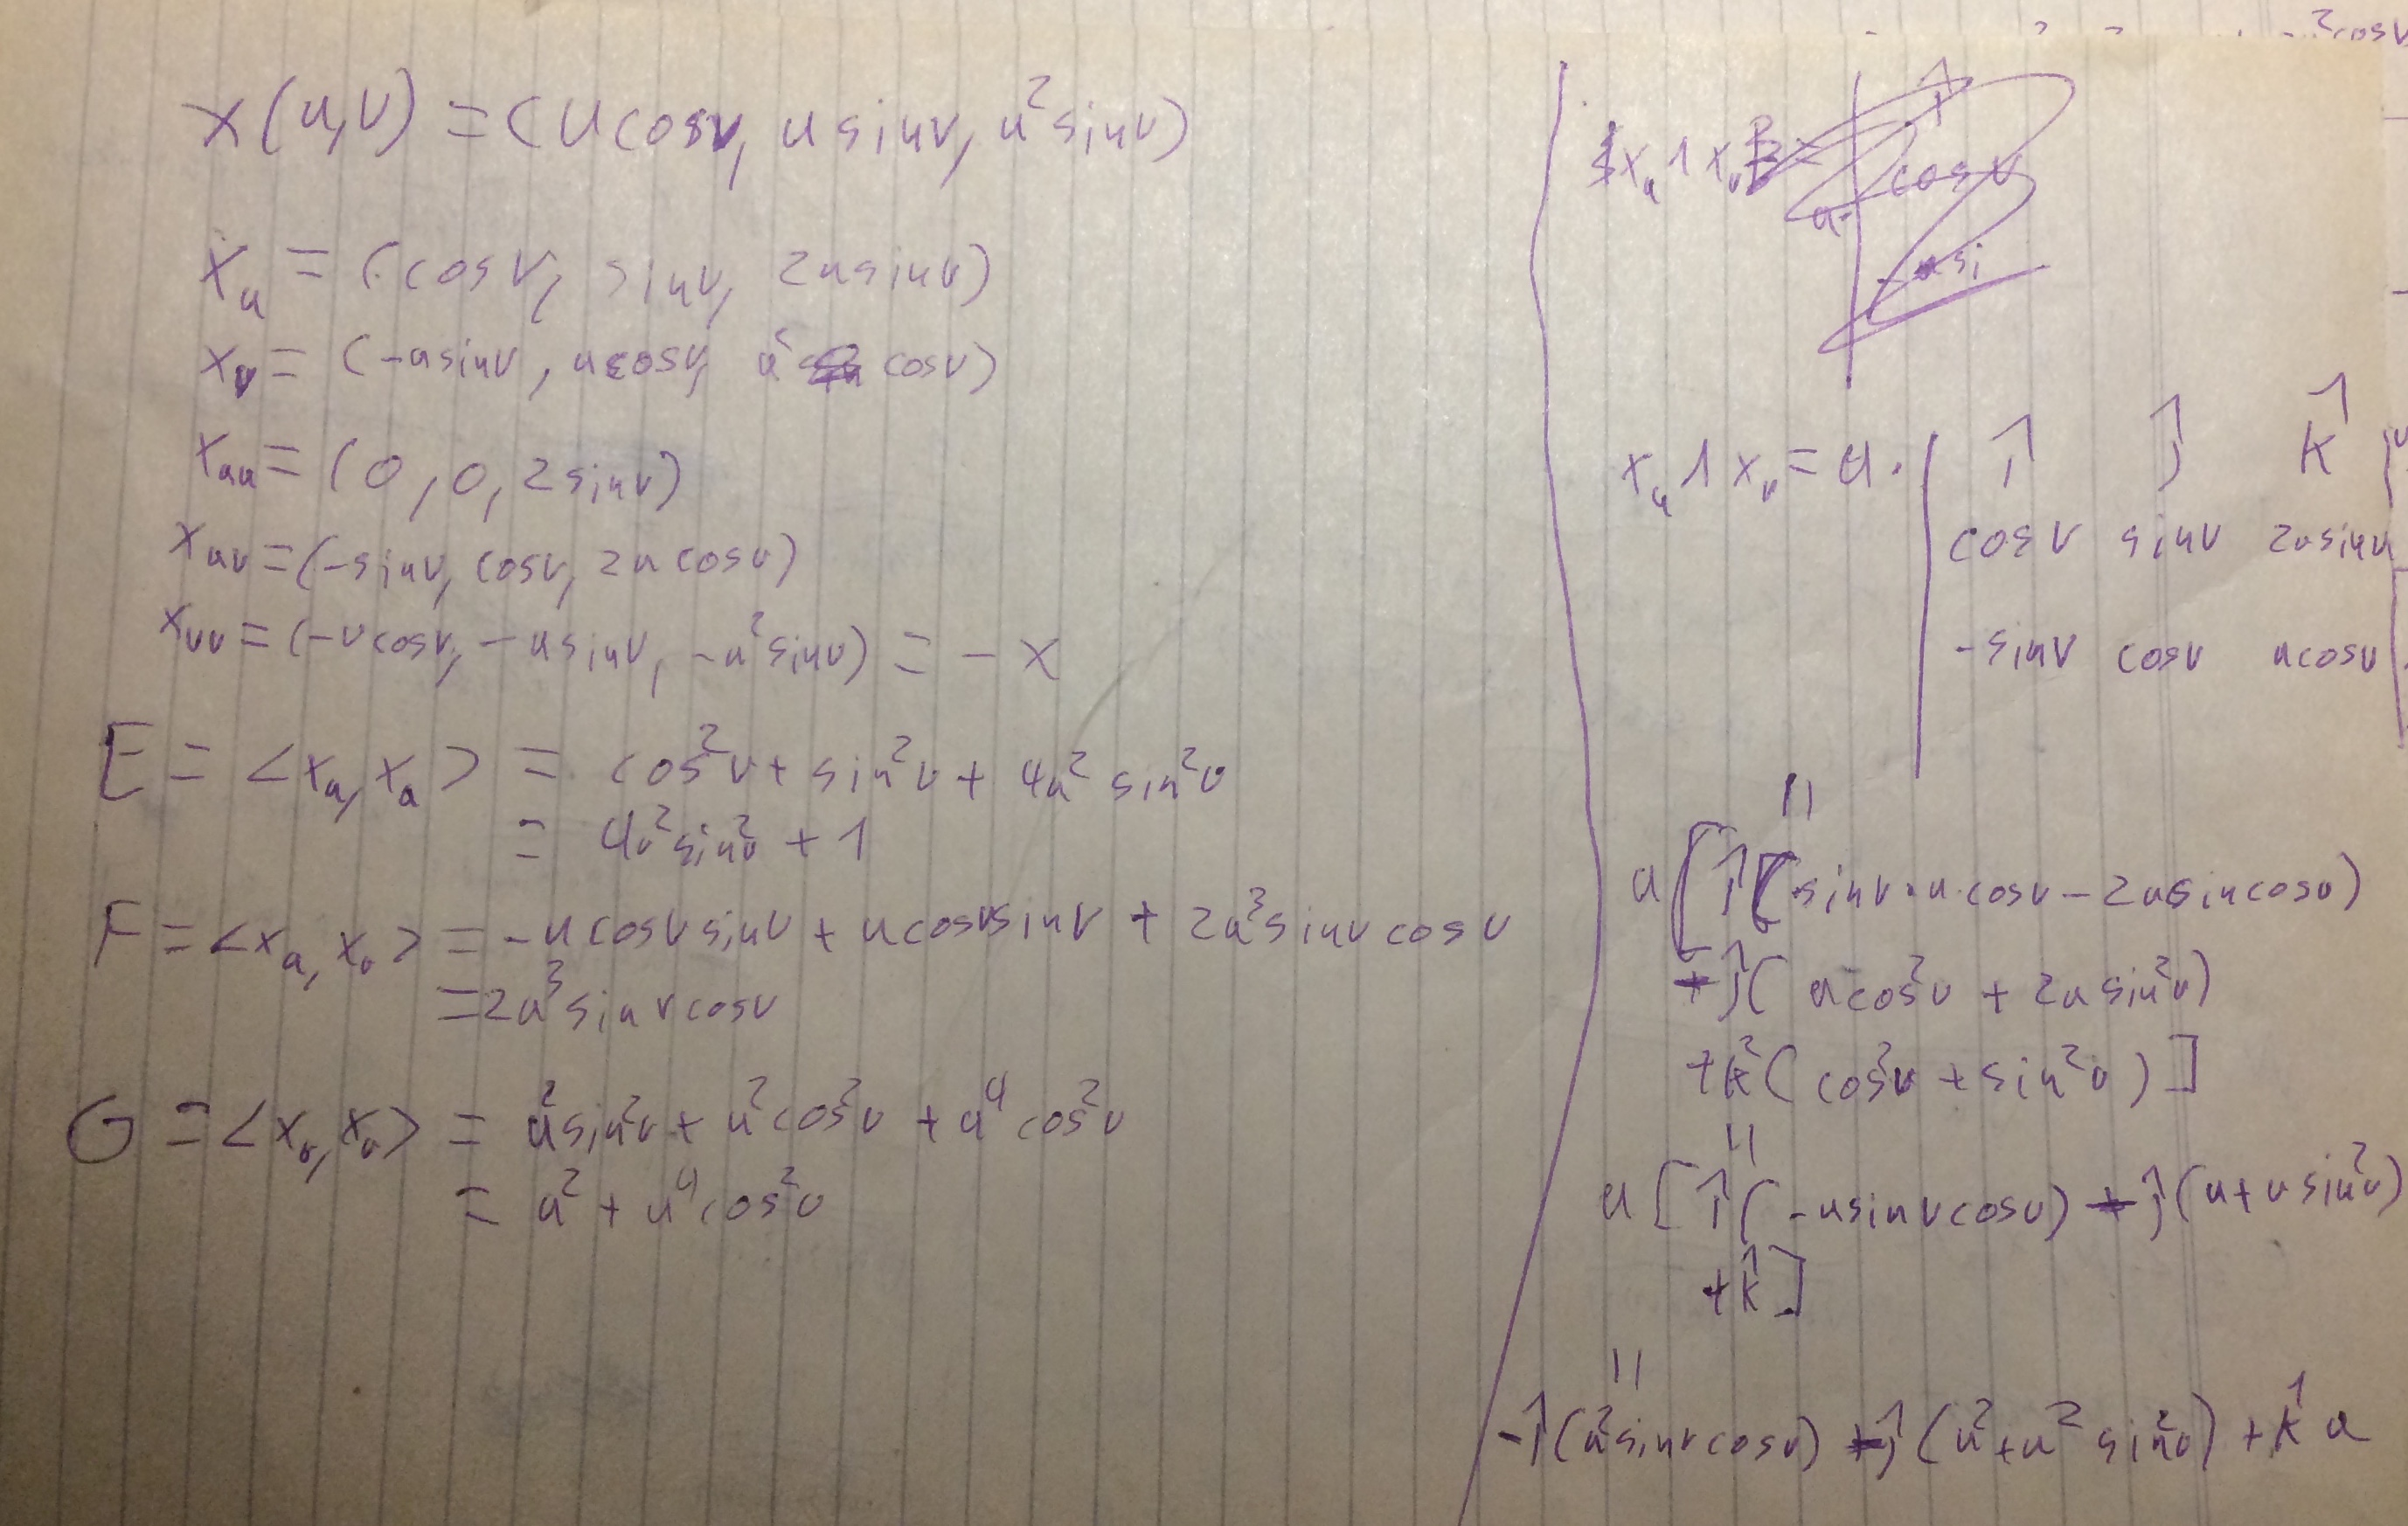
\includegraphics{img/IMG_5982.JPG}
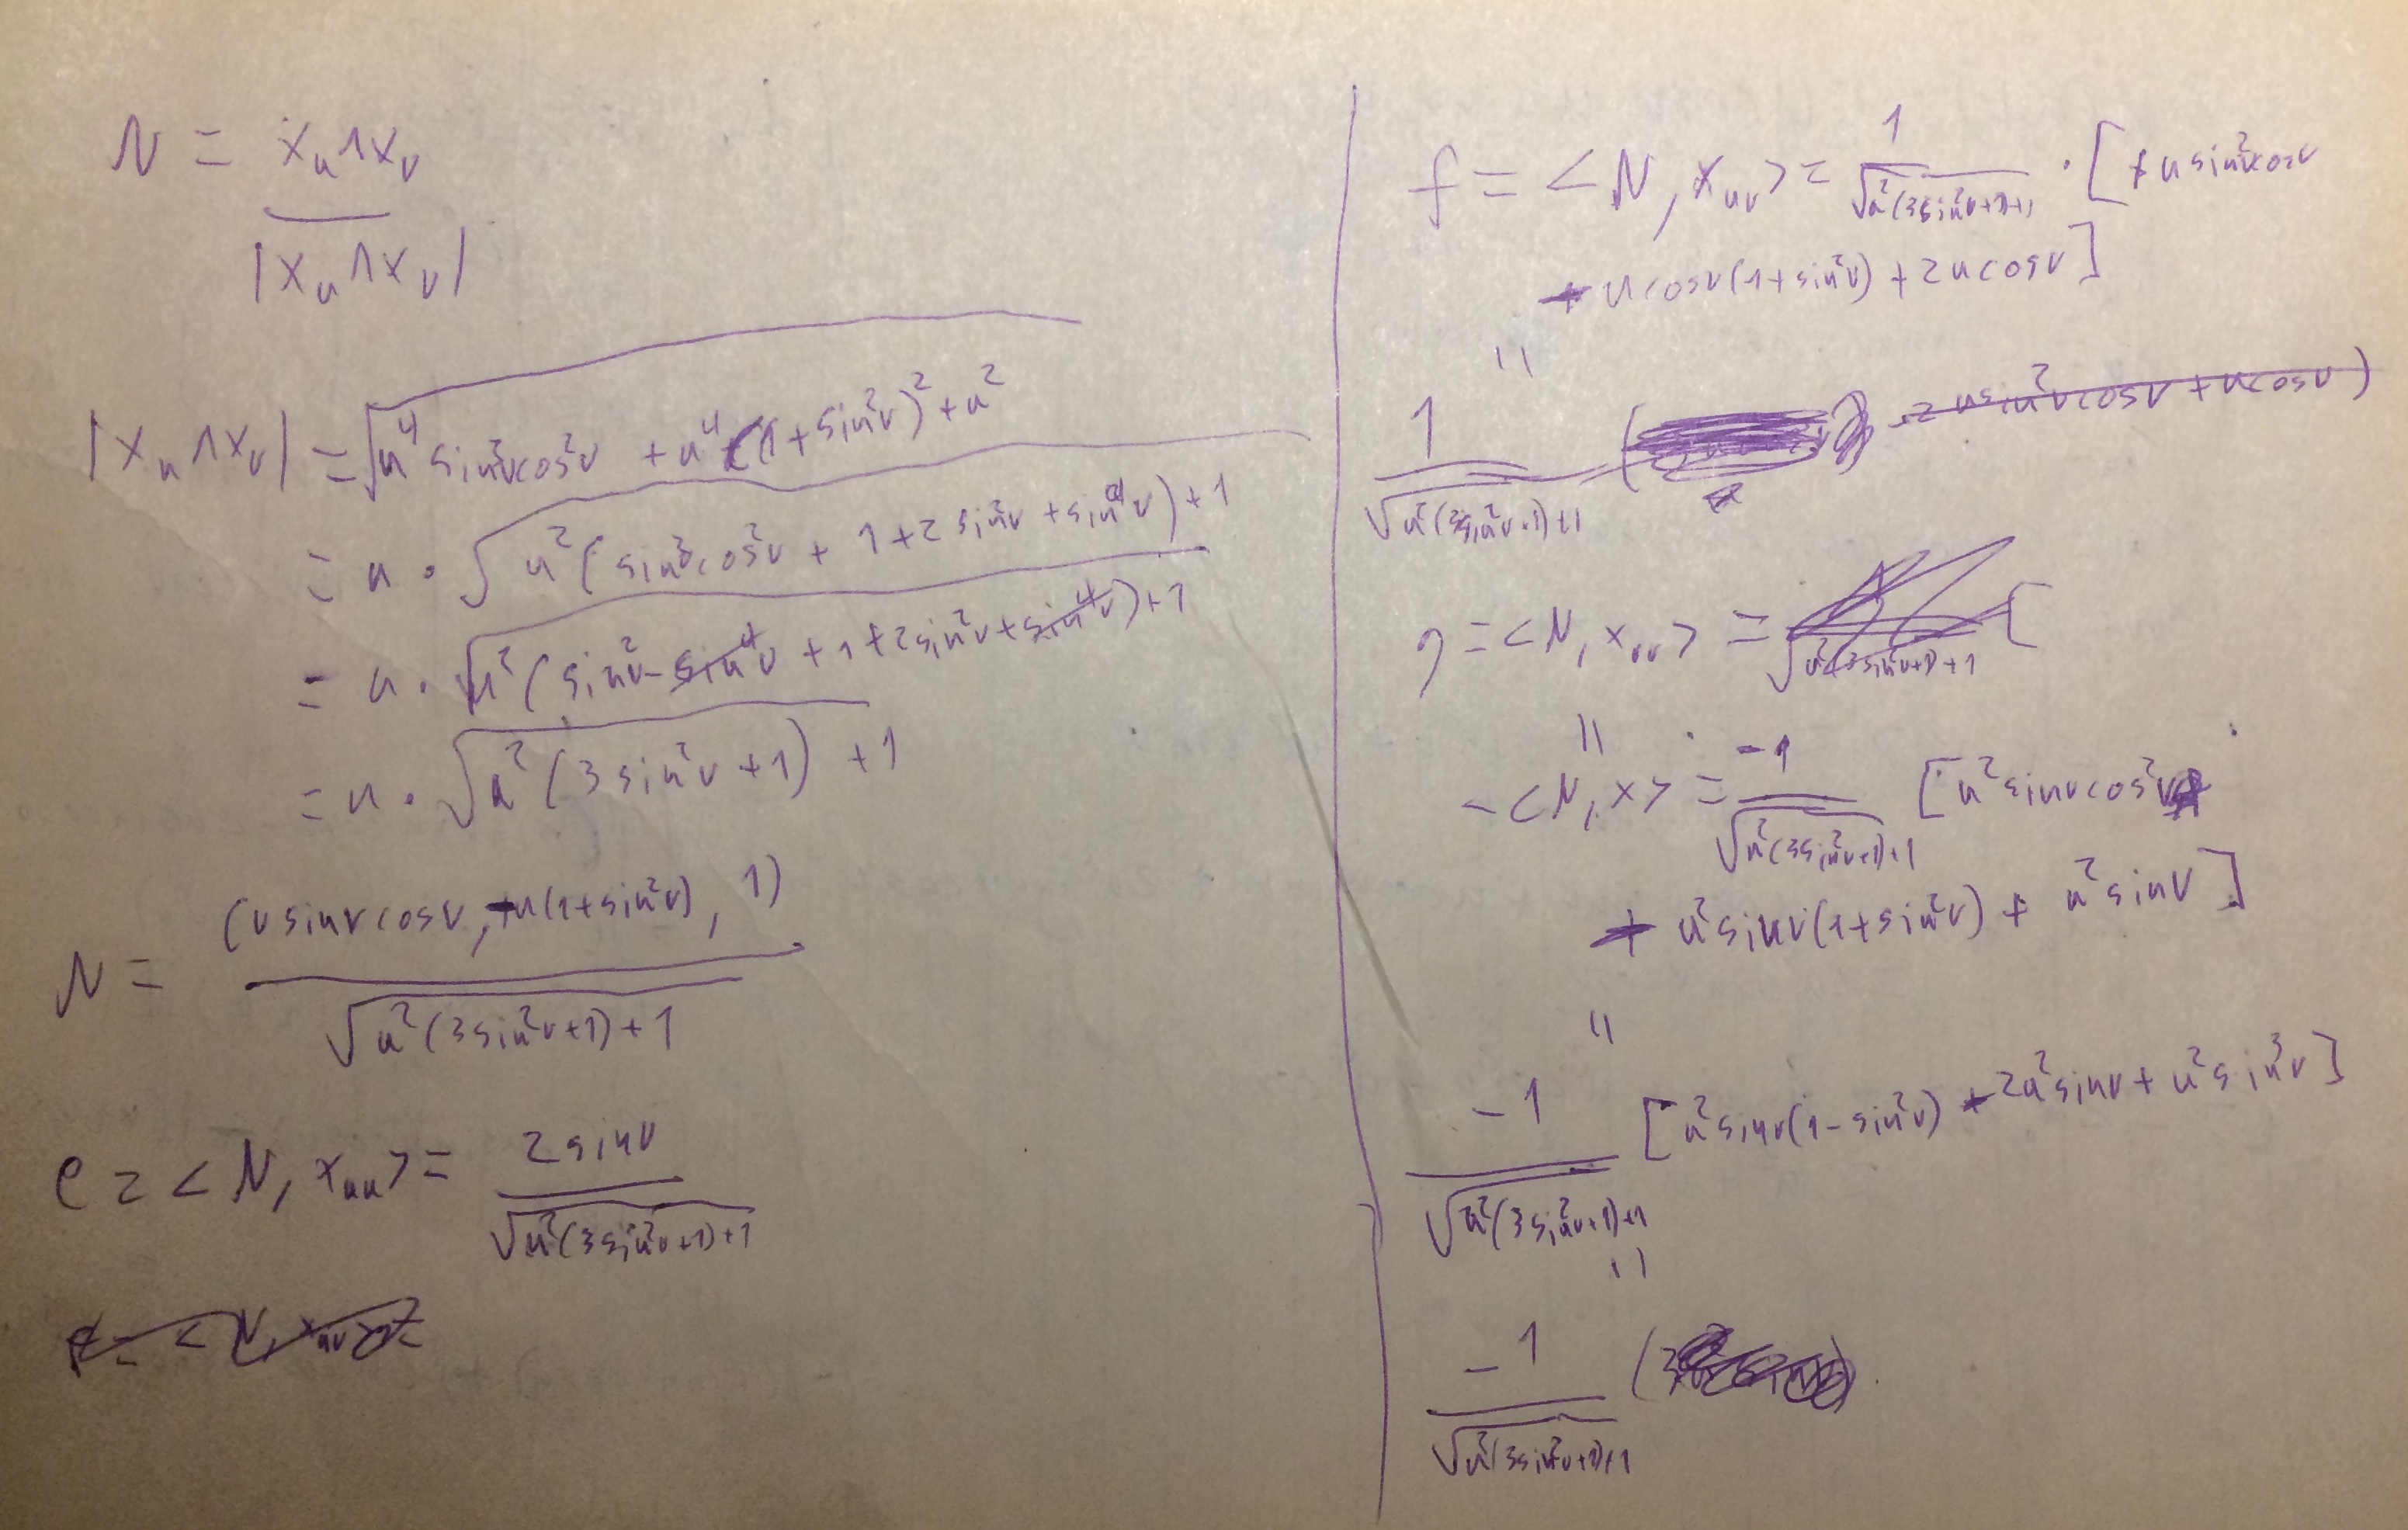
\includegraphics{img/IMG_5983.JPG}
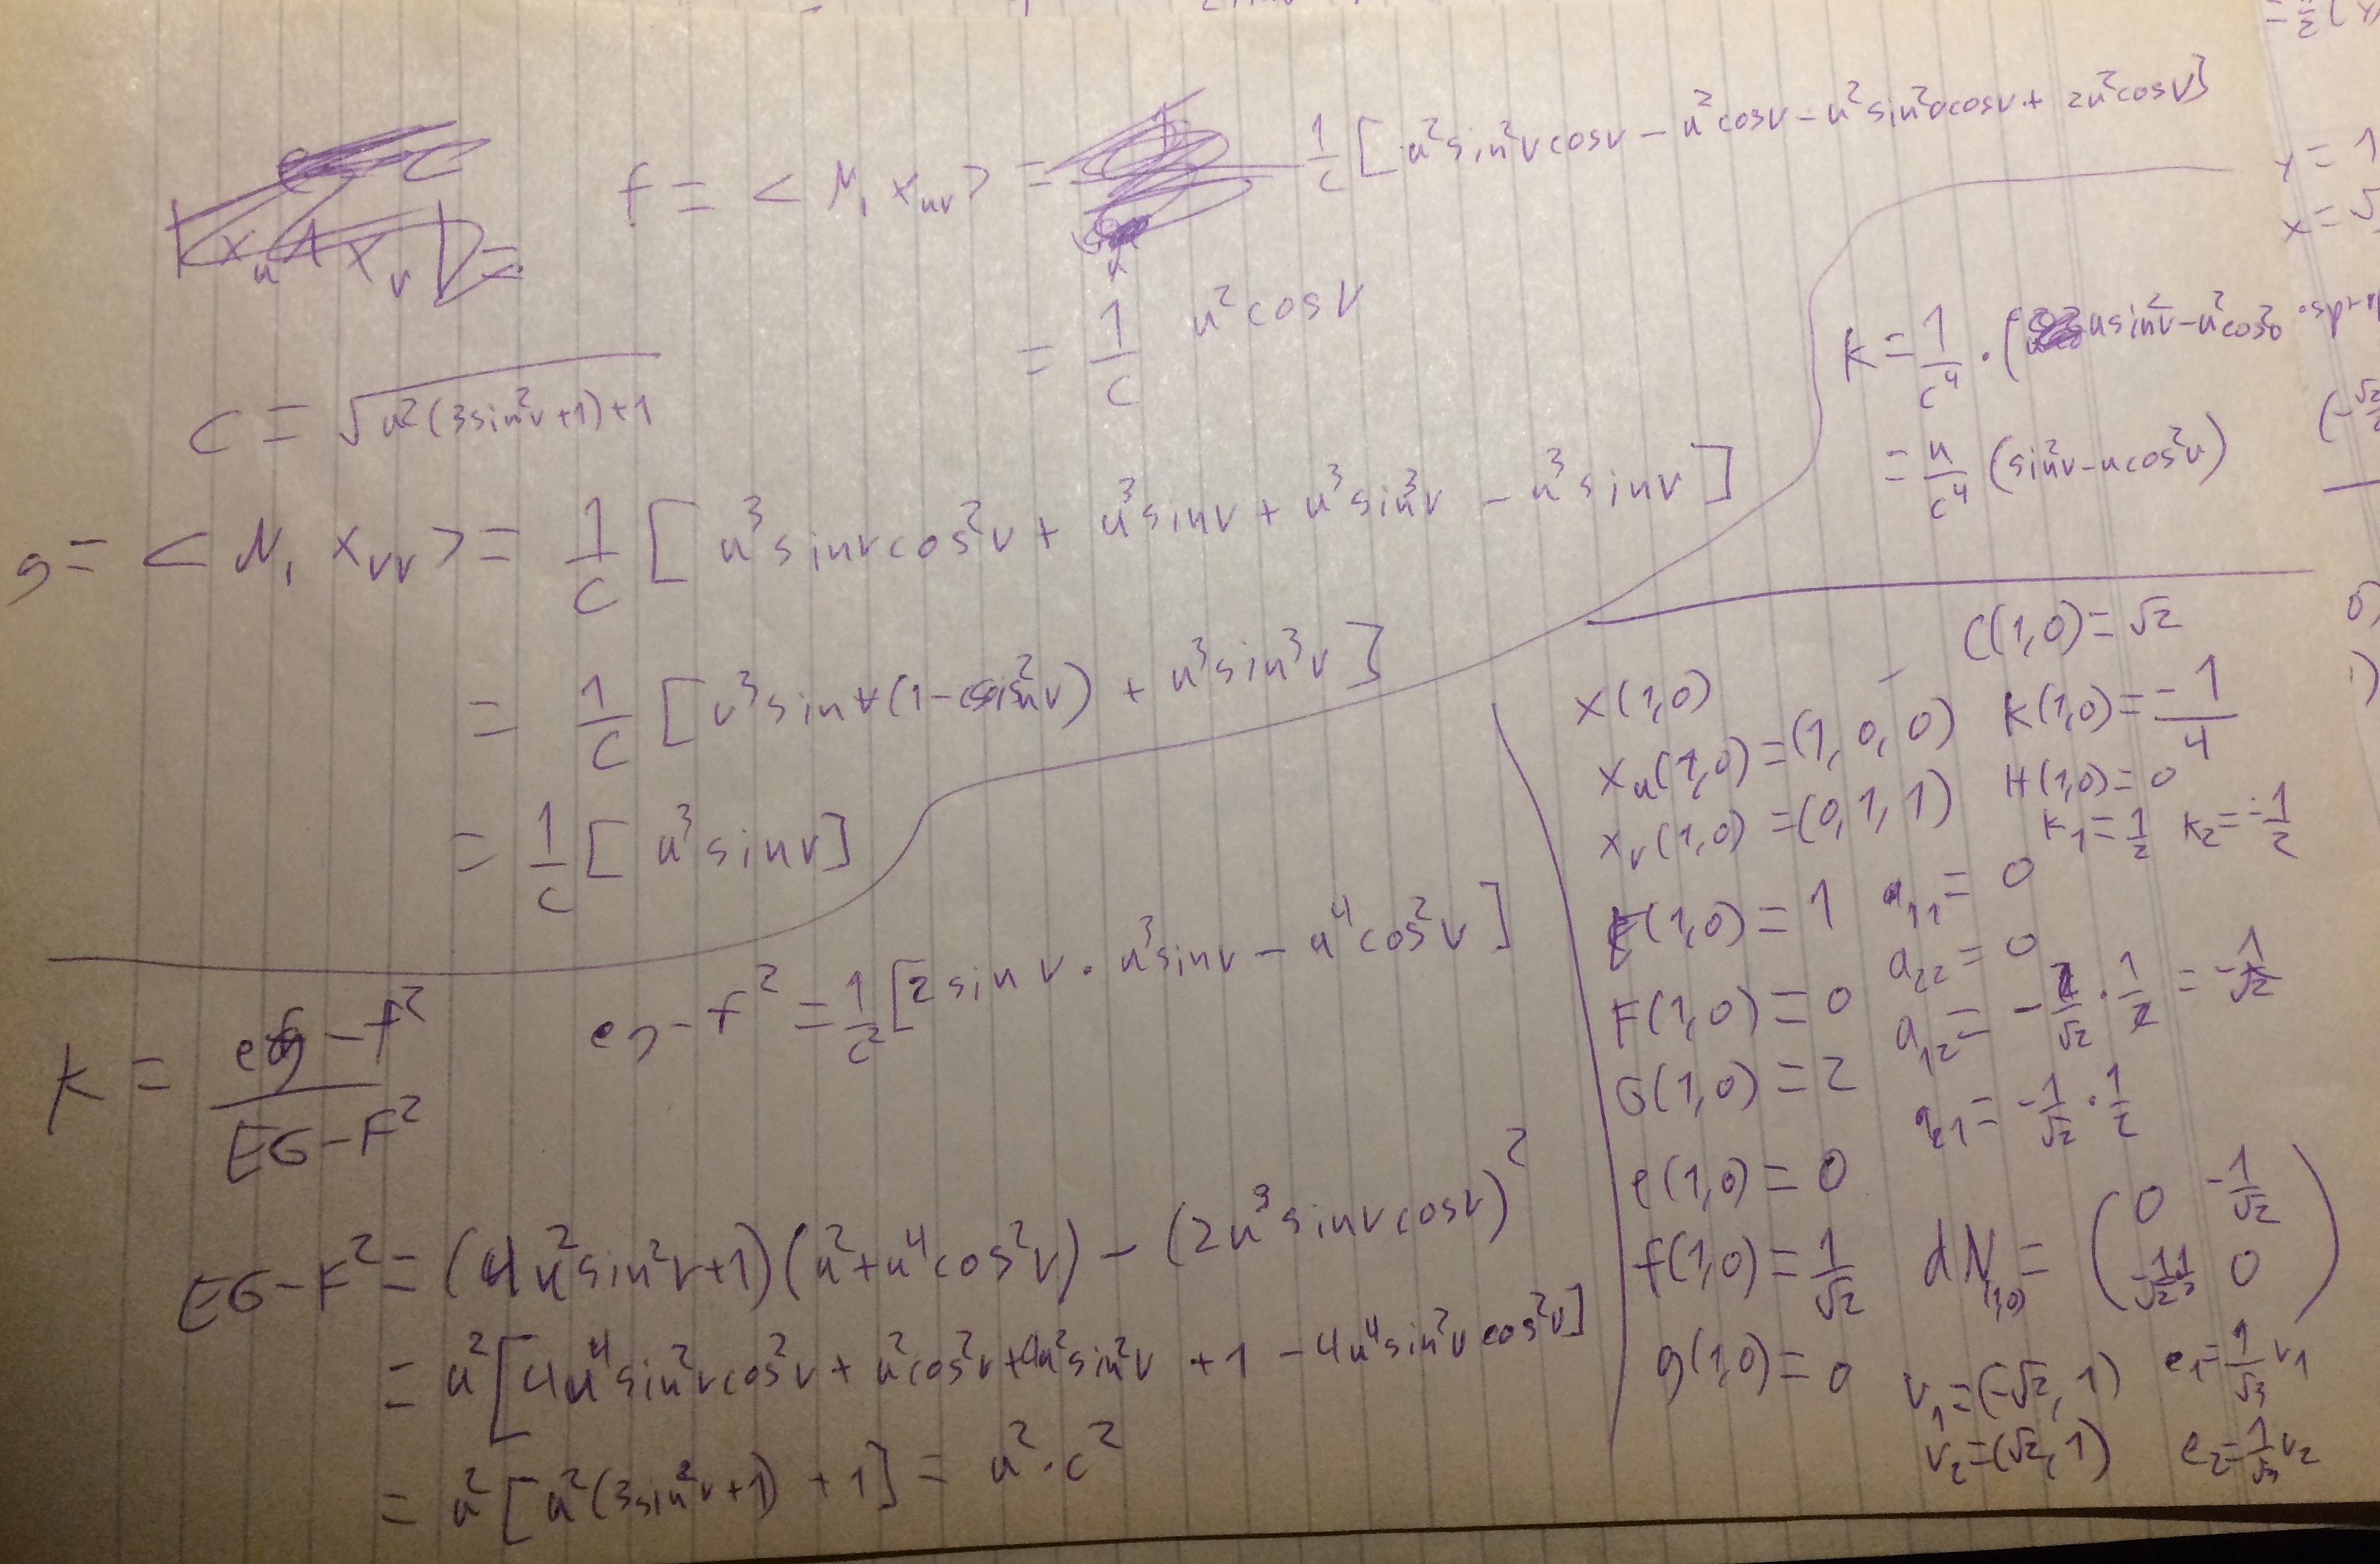
\includegraphics{img/IMG_5984.JPG}
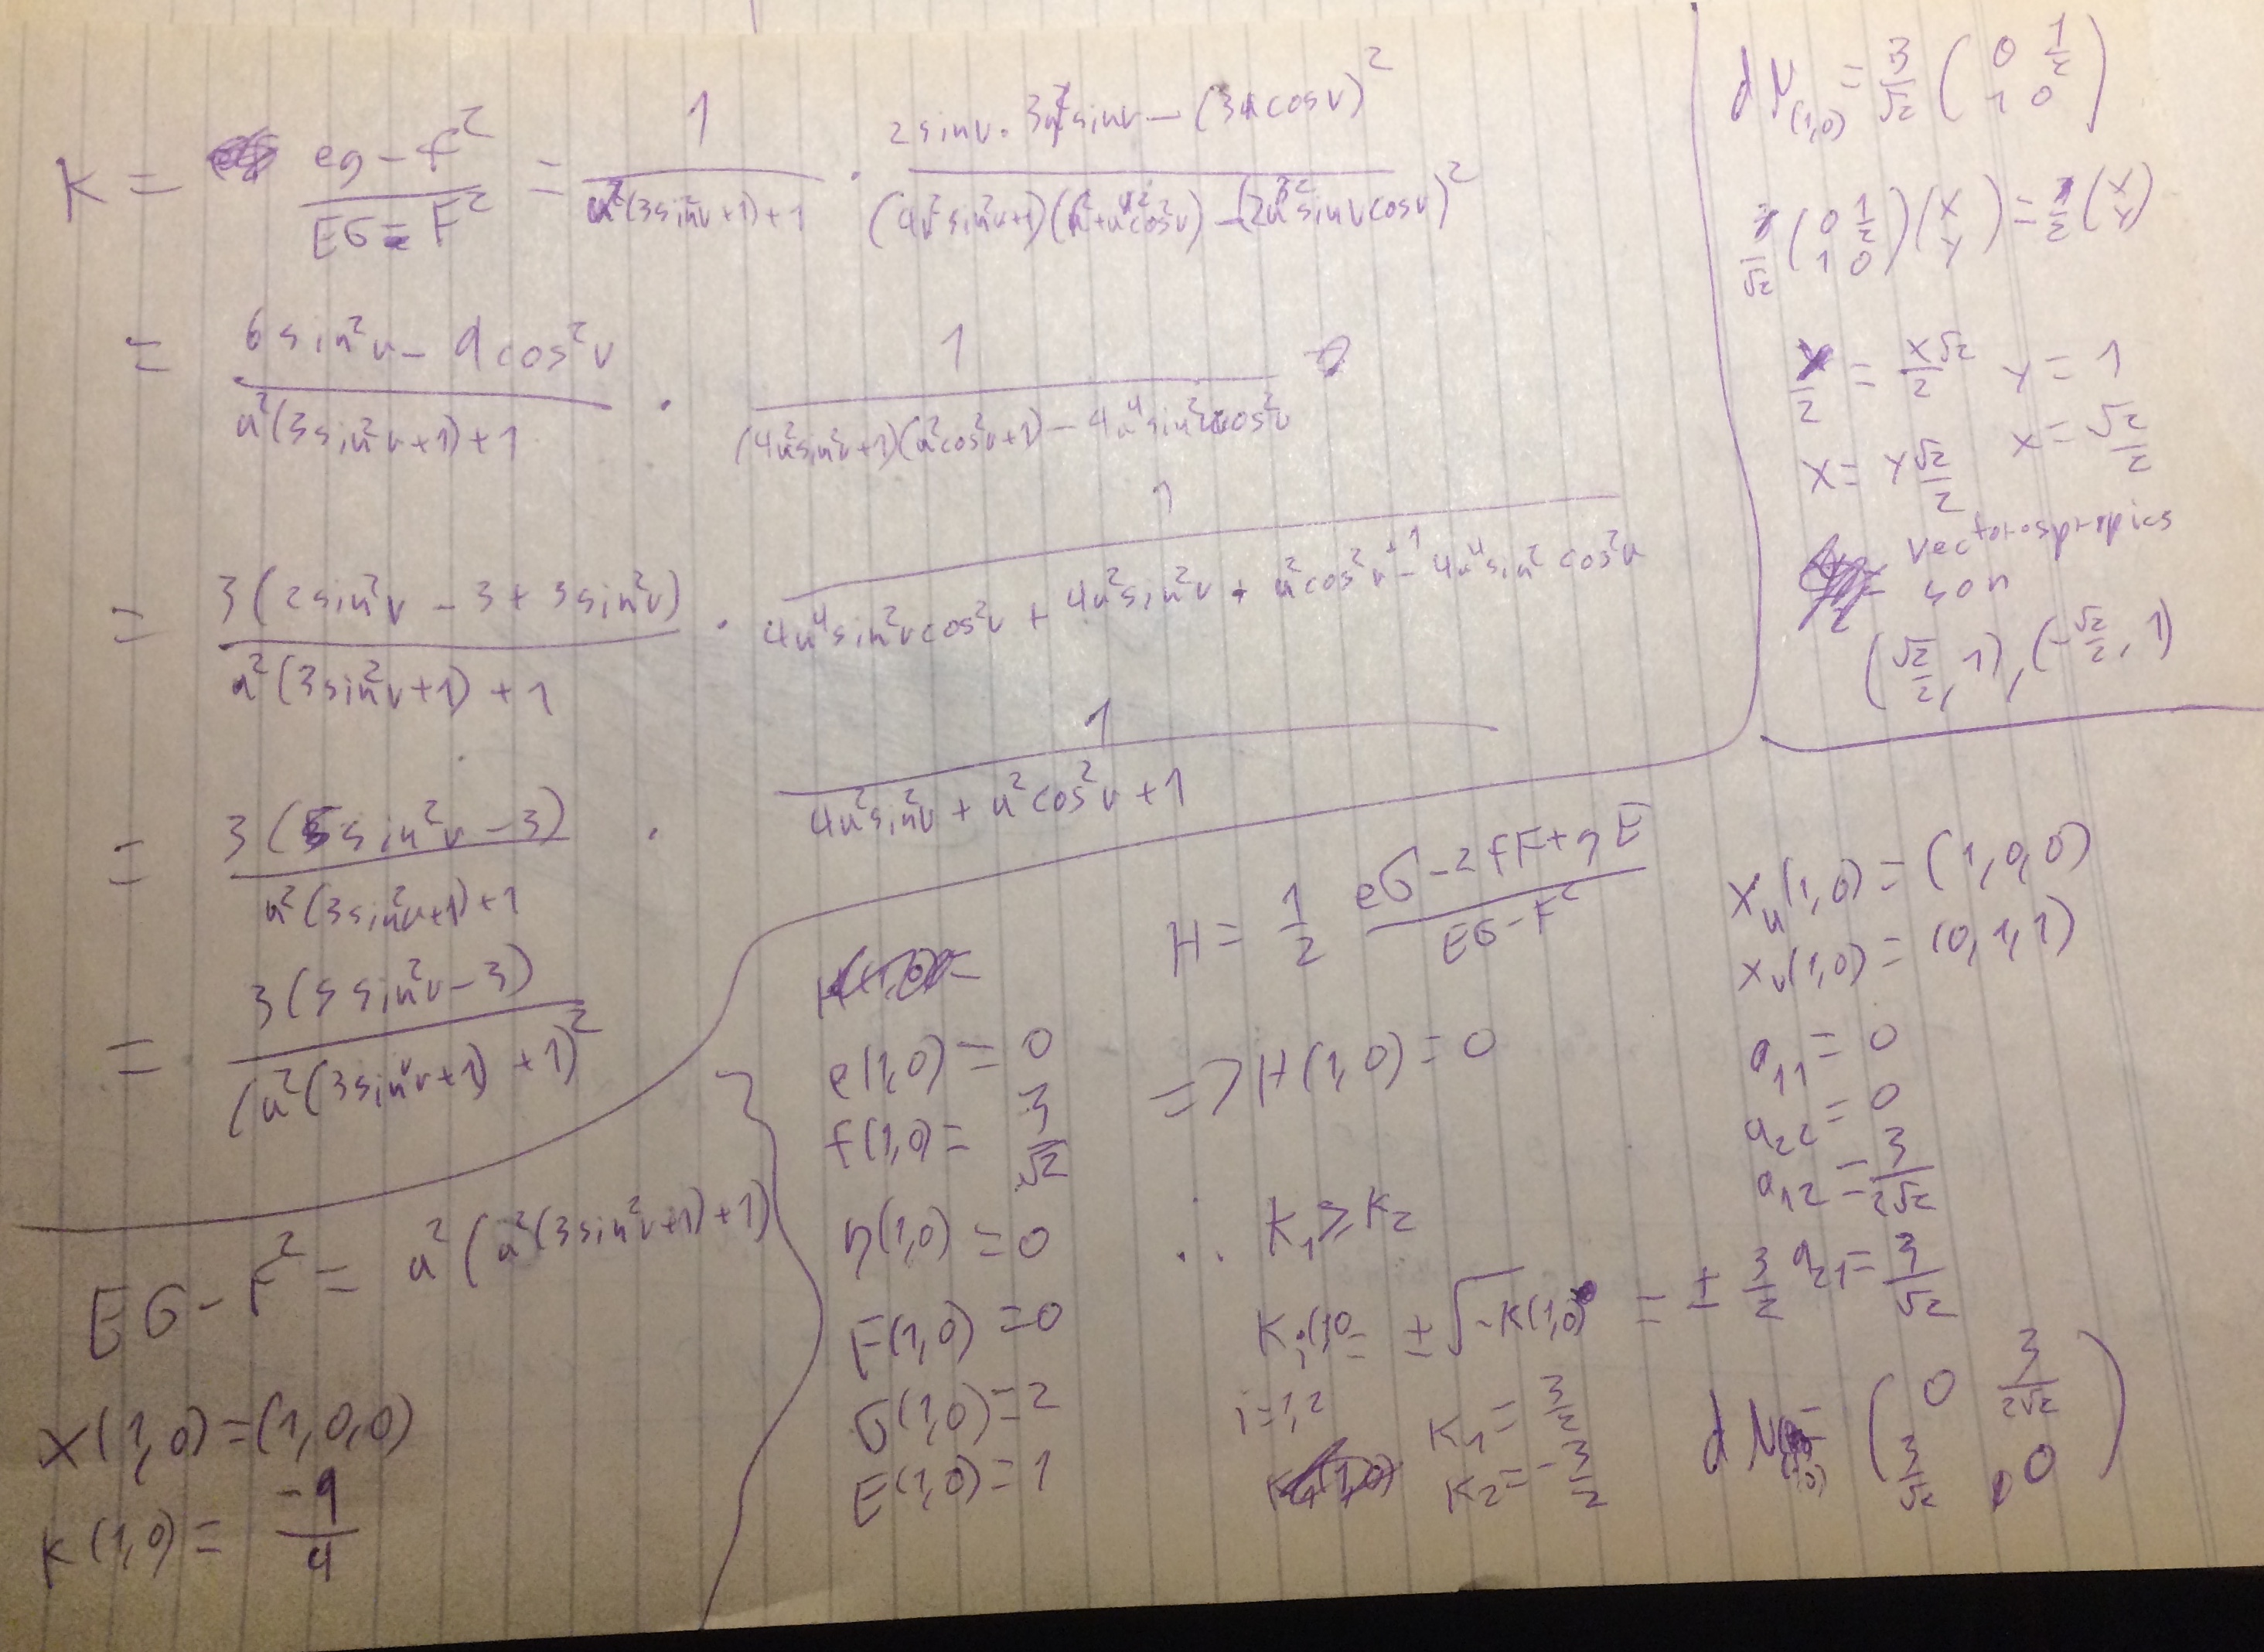
\includegraphics{img/IMG_5985.JPG}
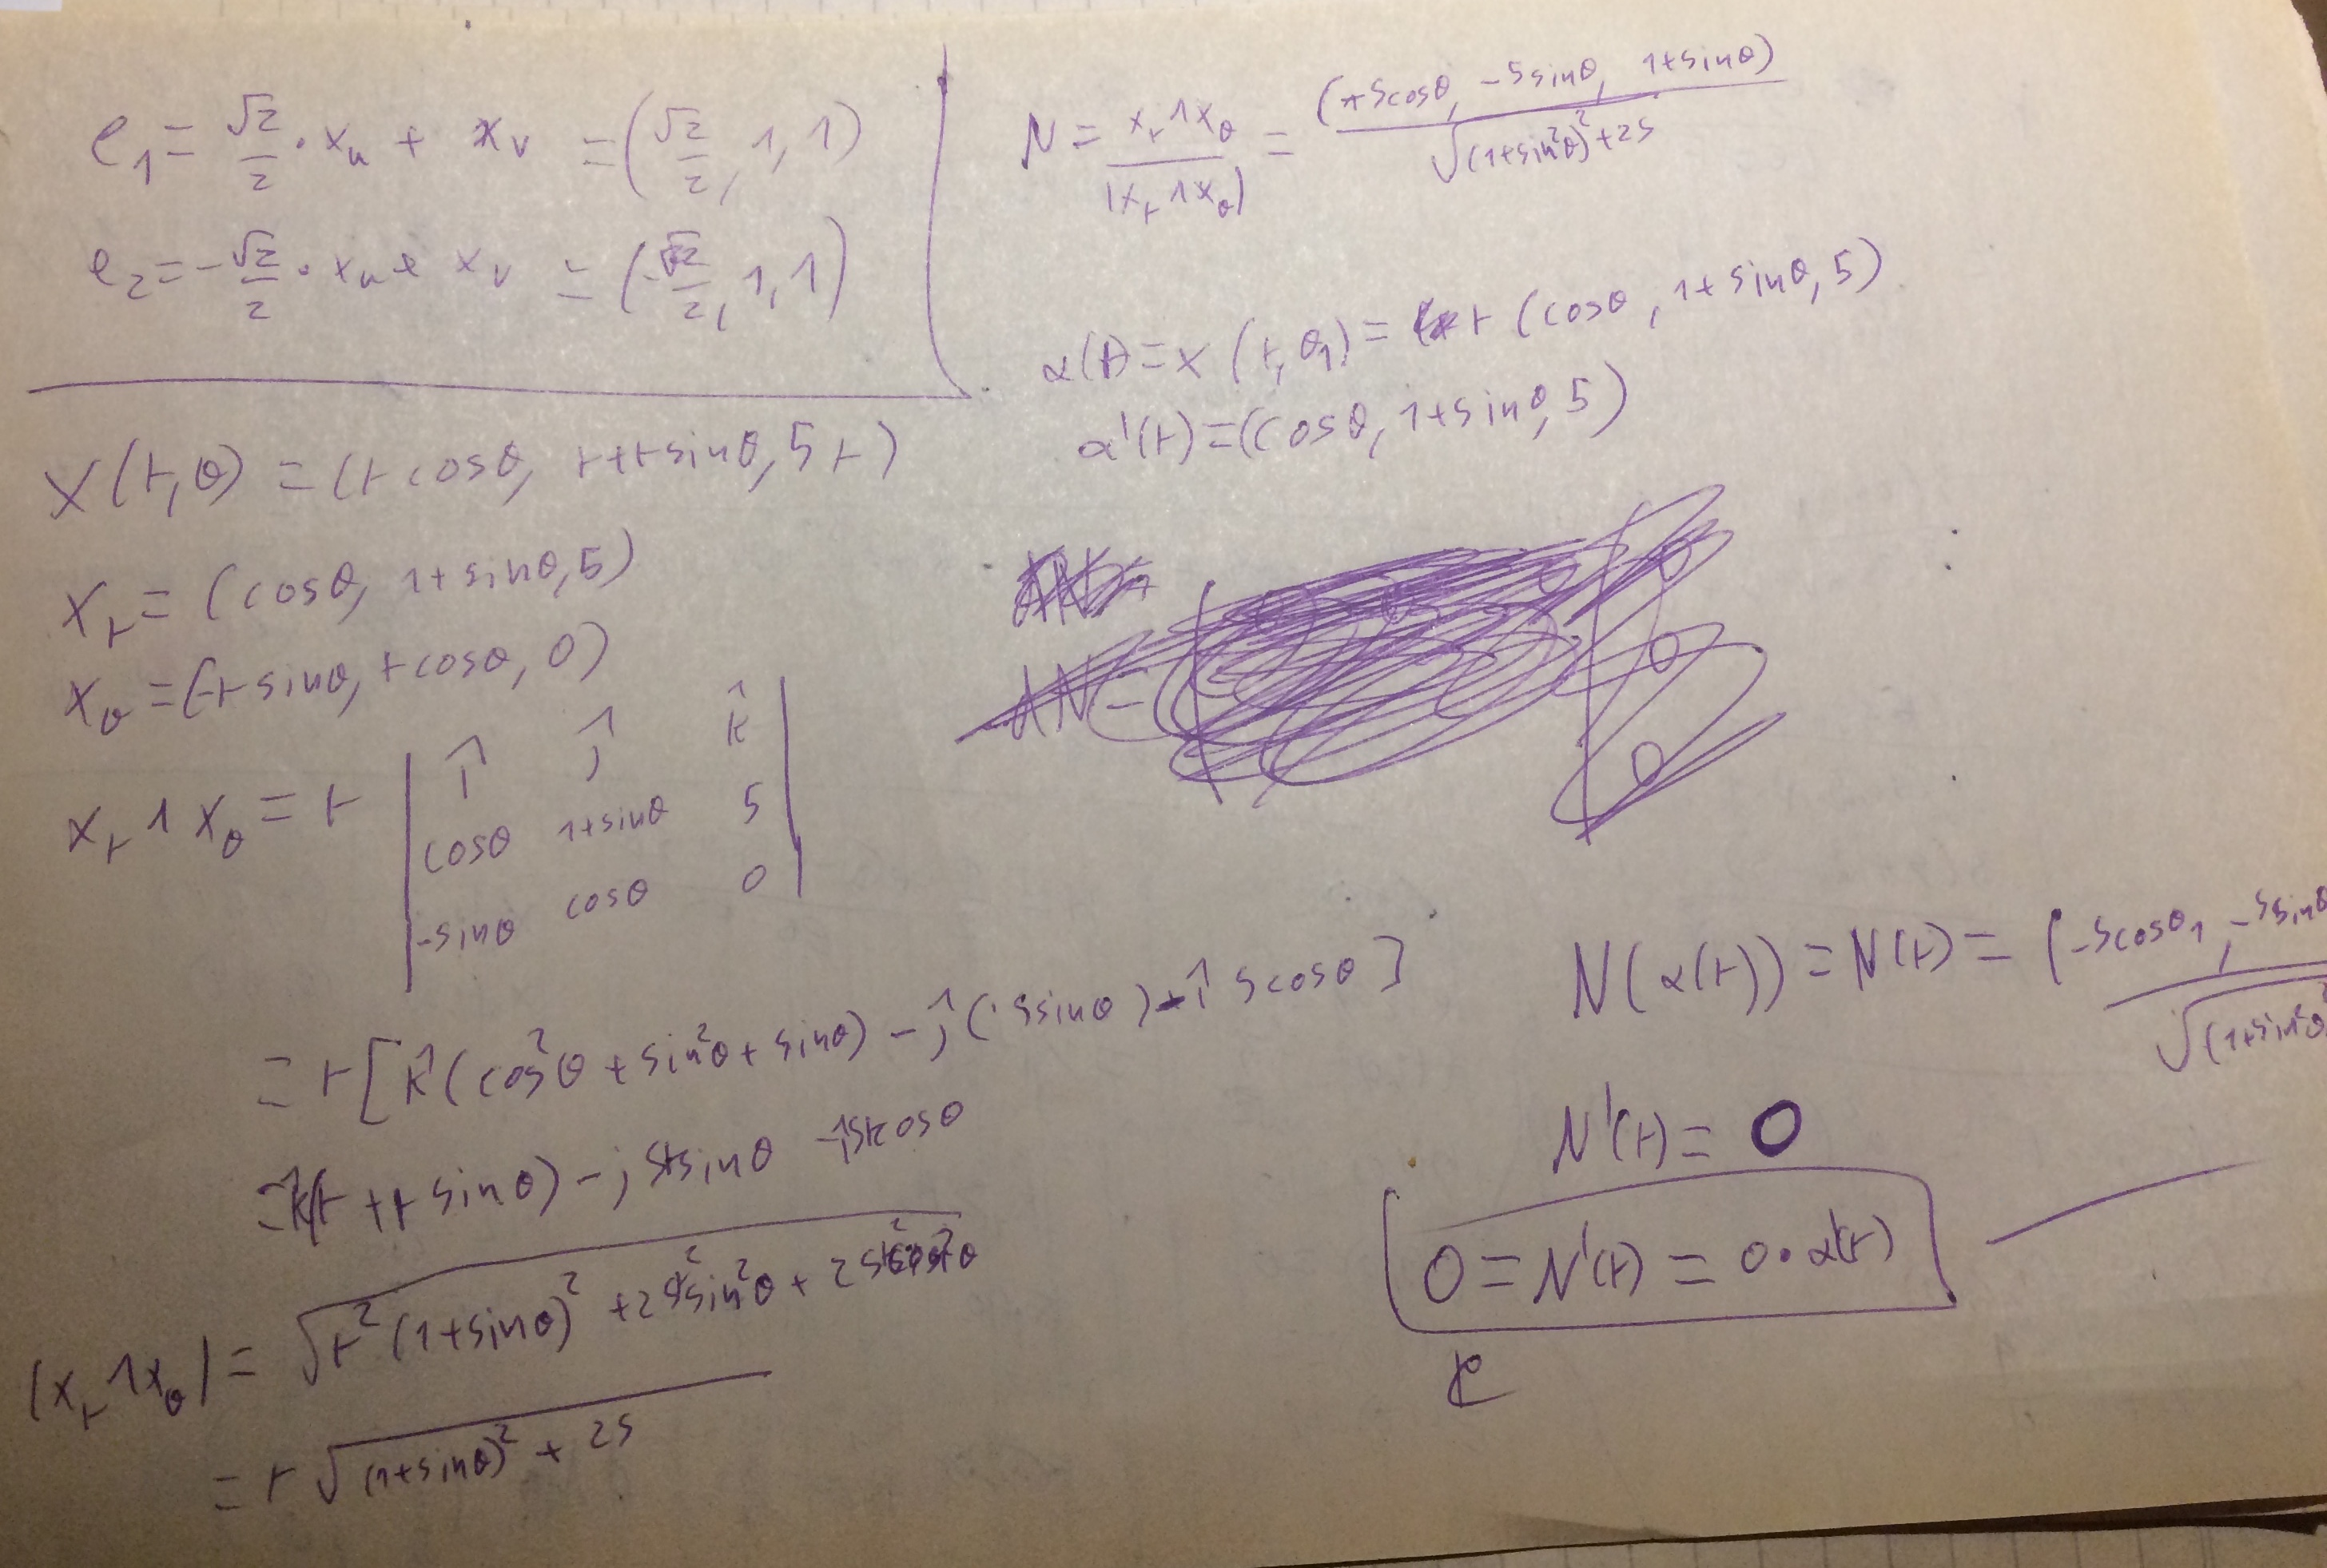
\includegraphics{img/IMG_5986.JPG}
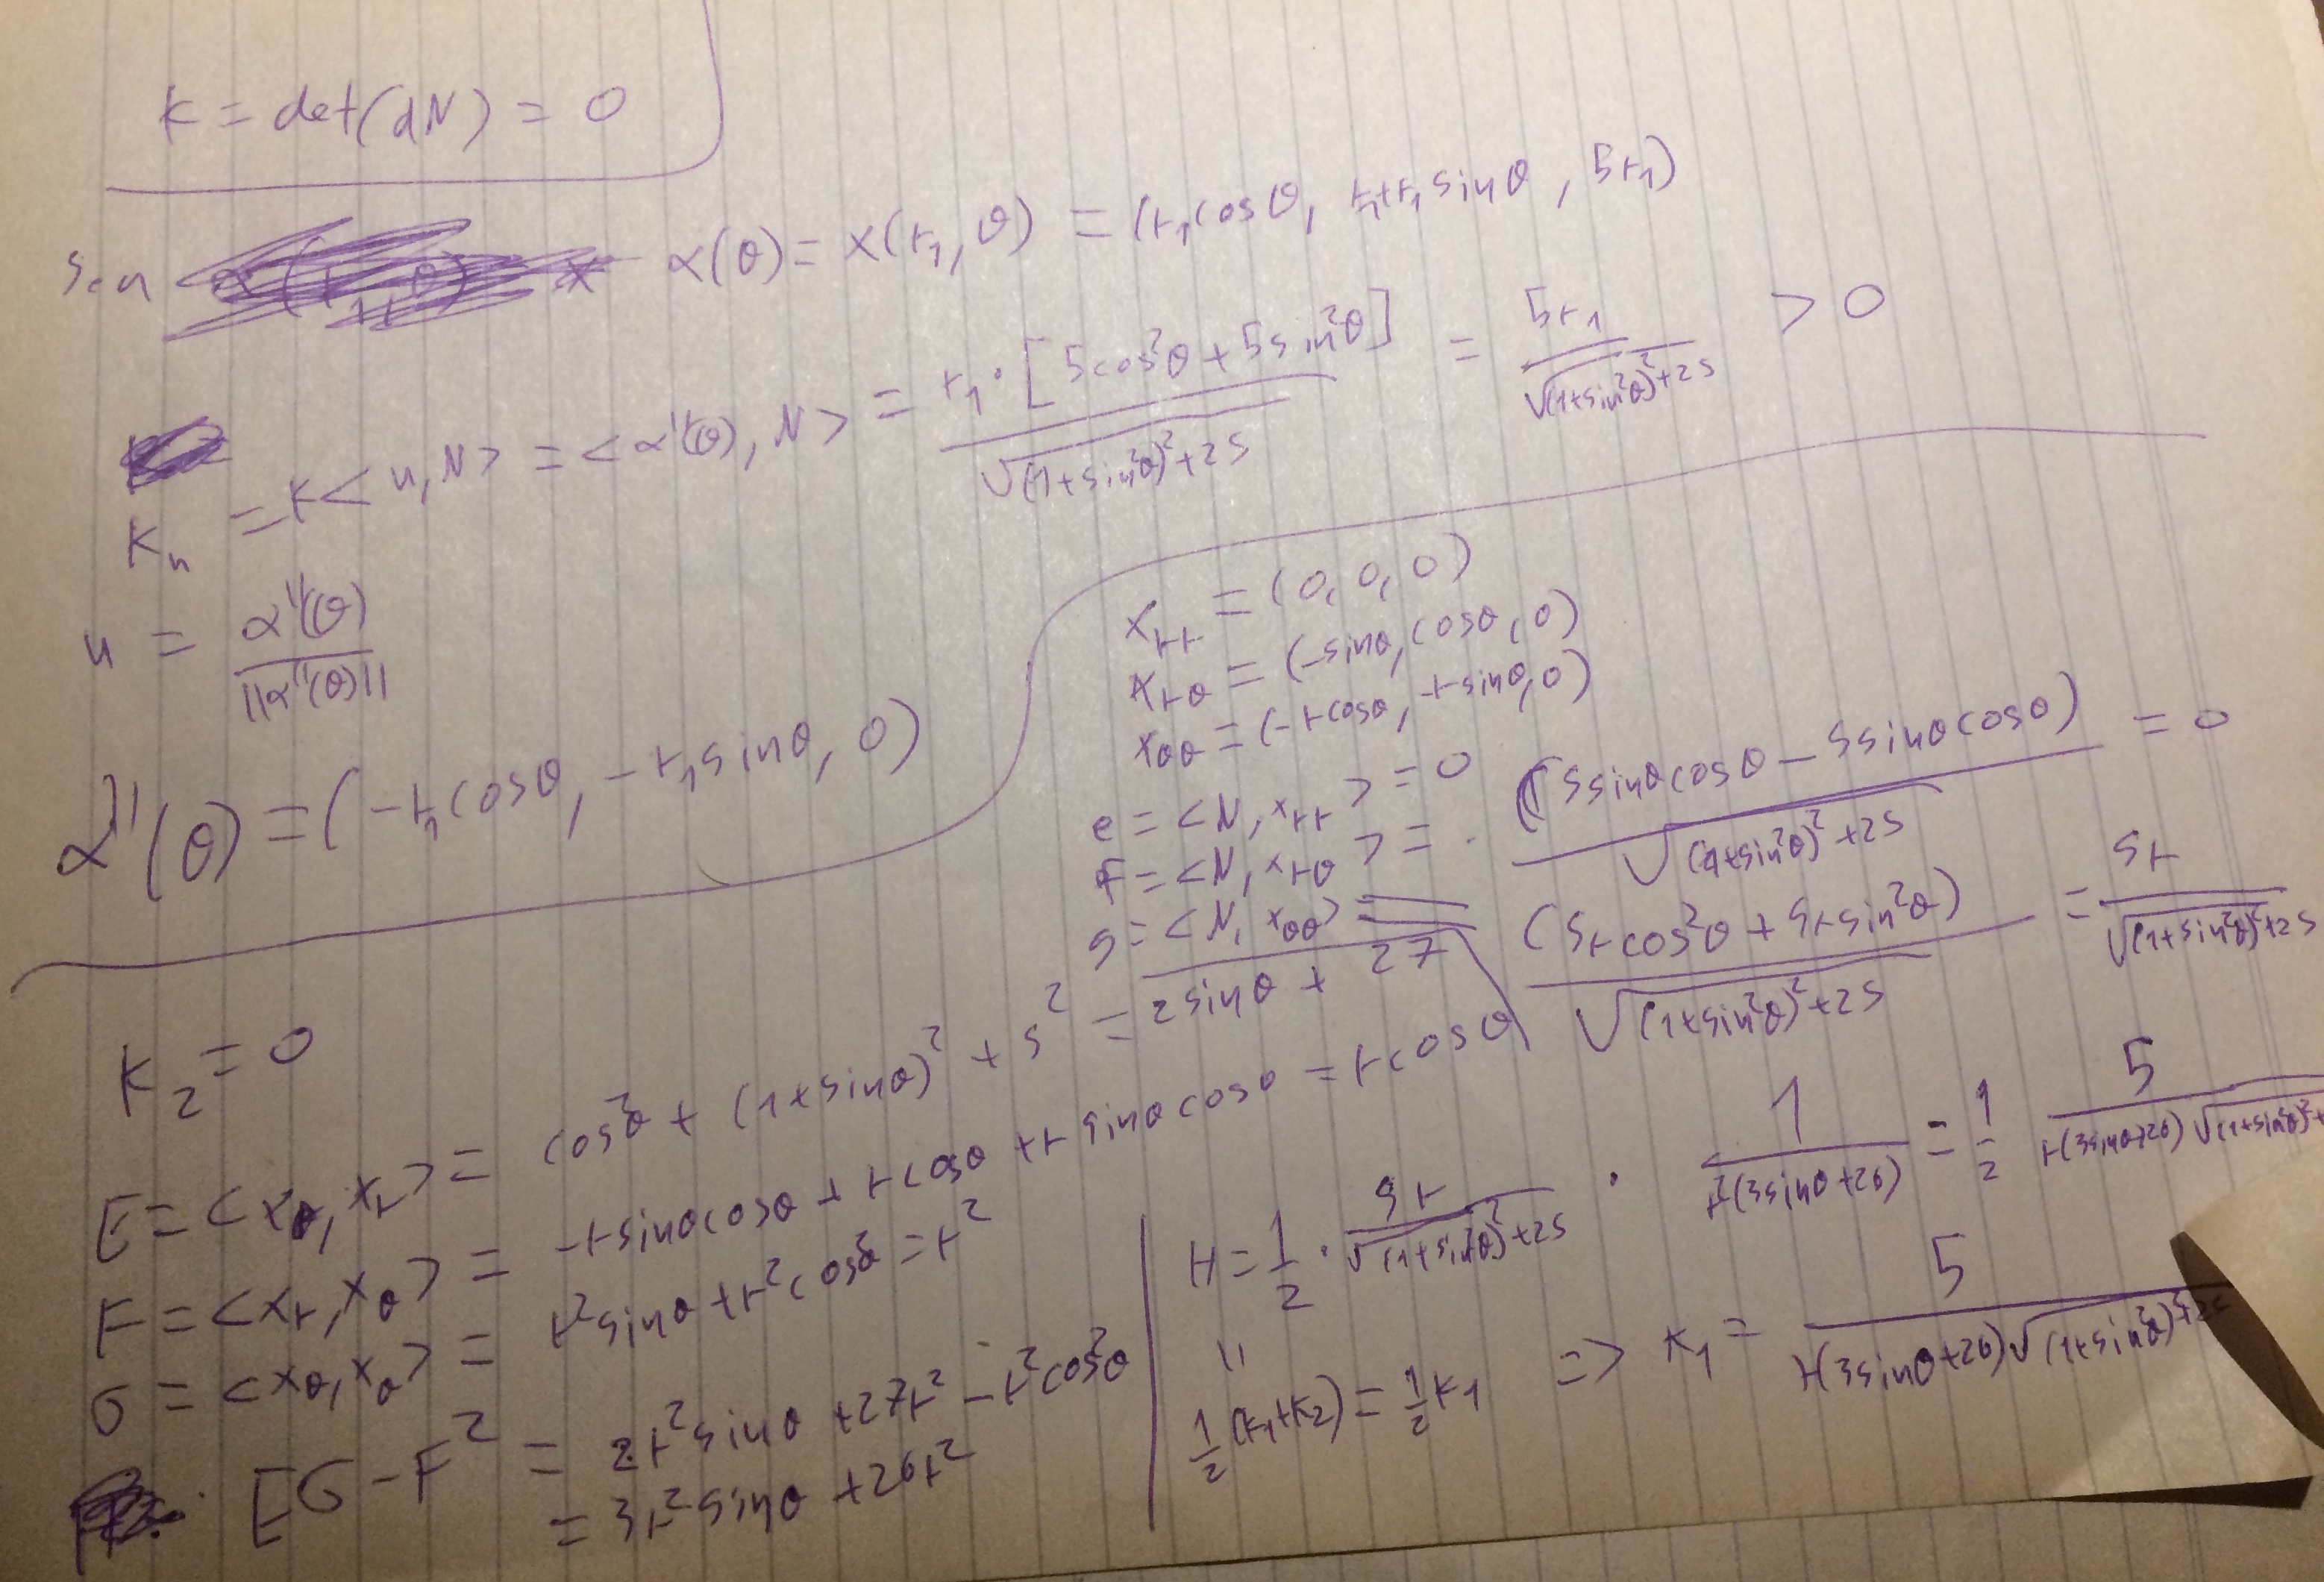
\includegraphics{img/IMG_5987.JPG}
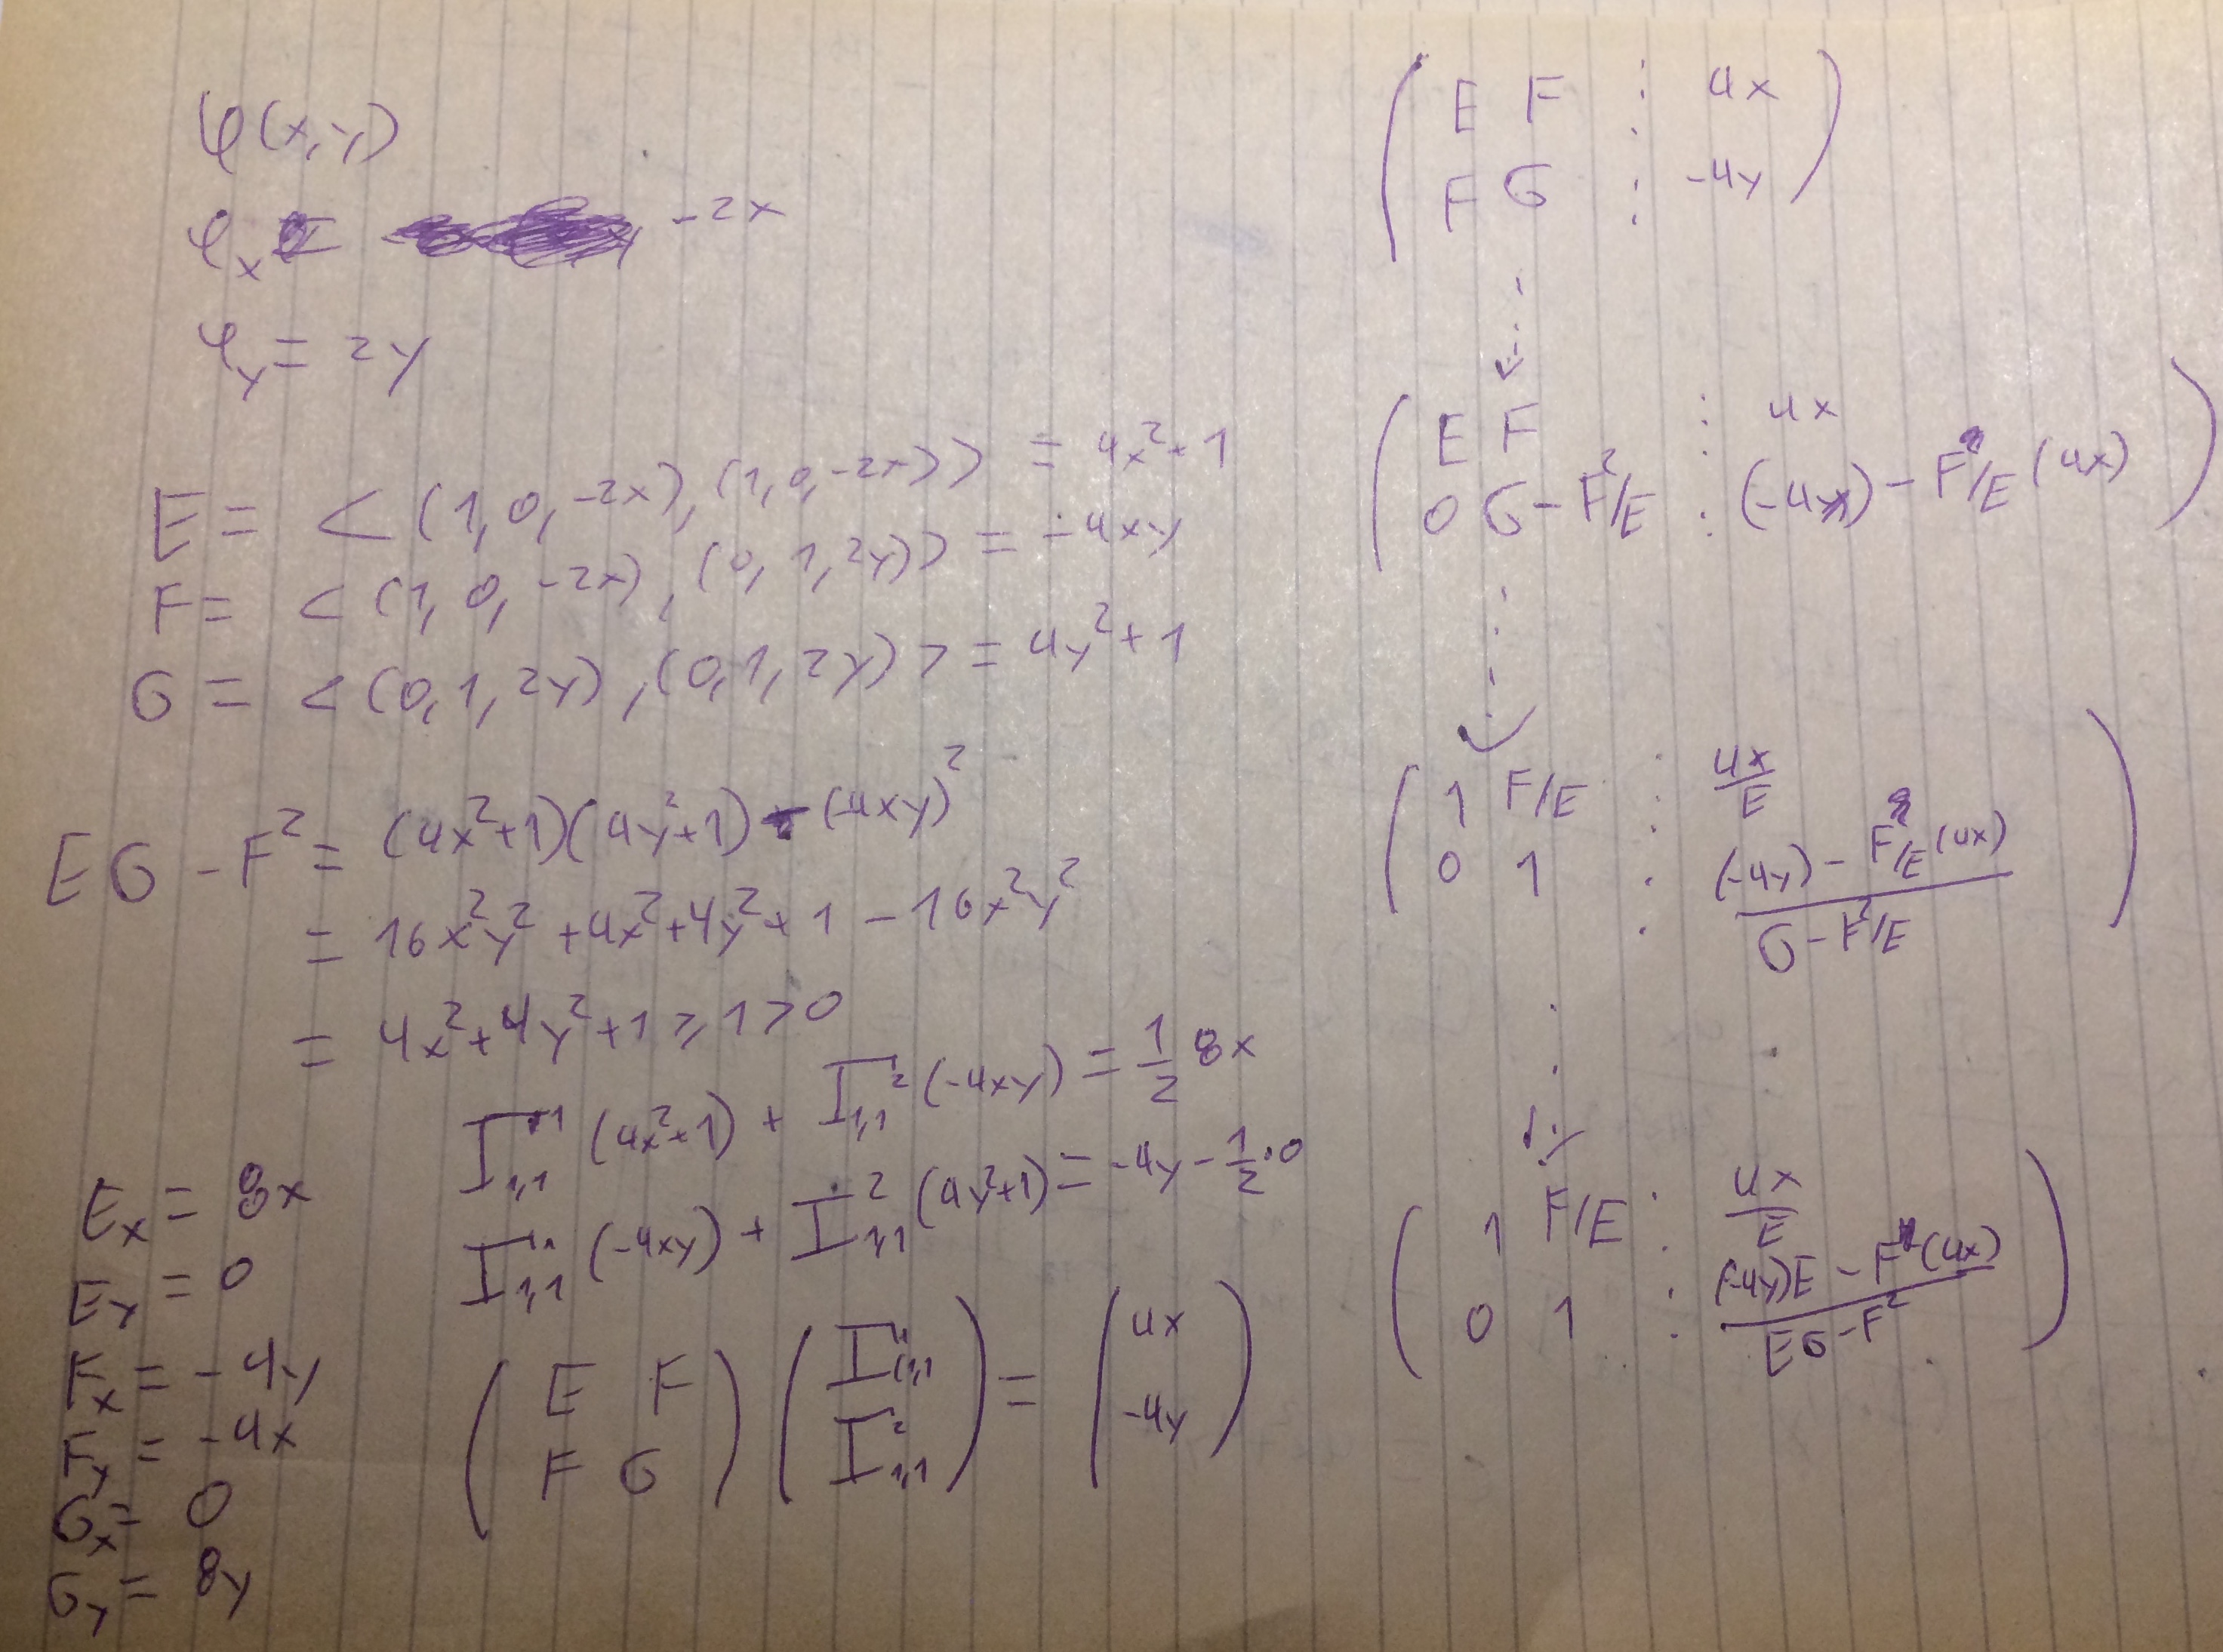
\includegraphics{img/IMG_5988.JPG}
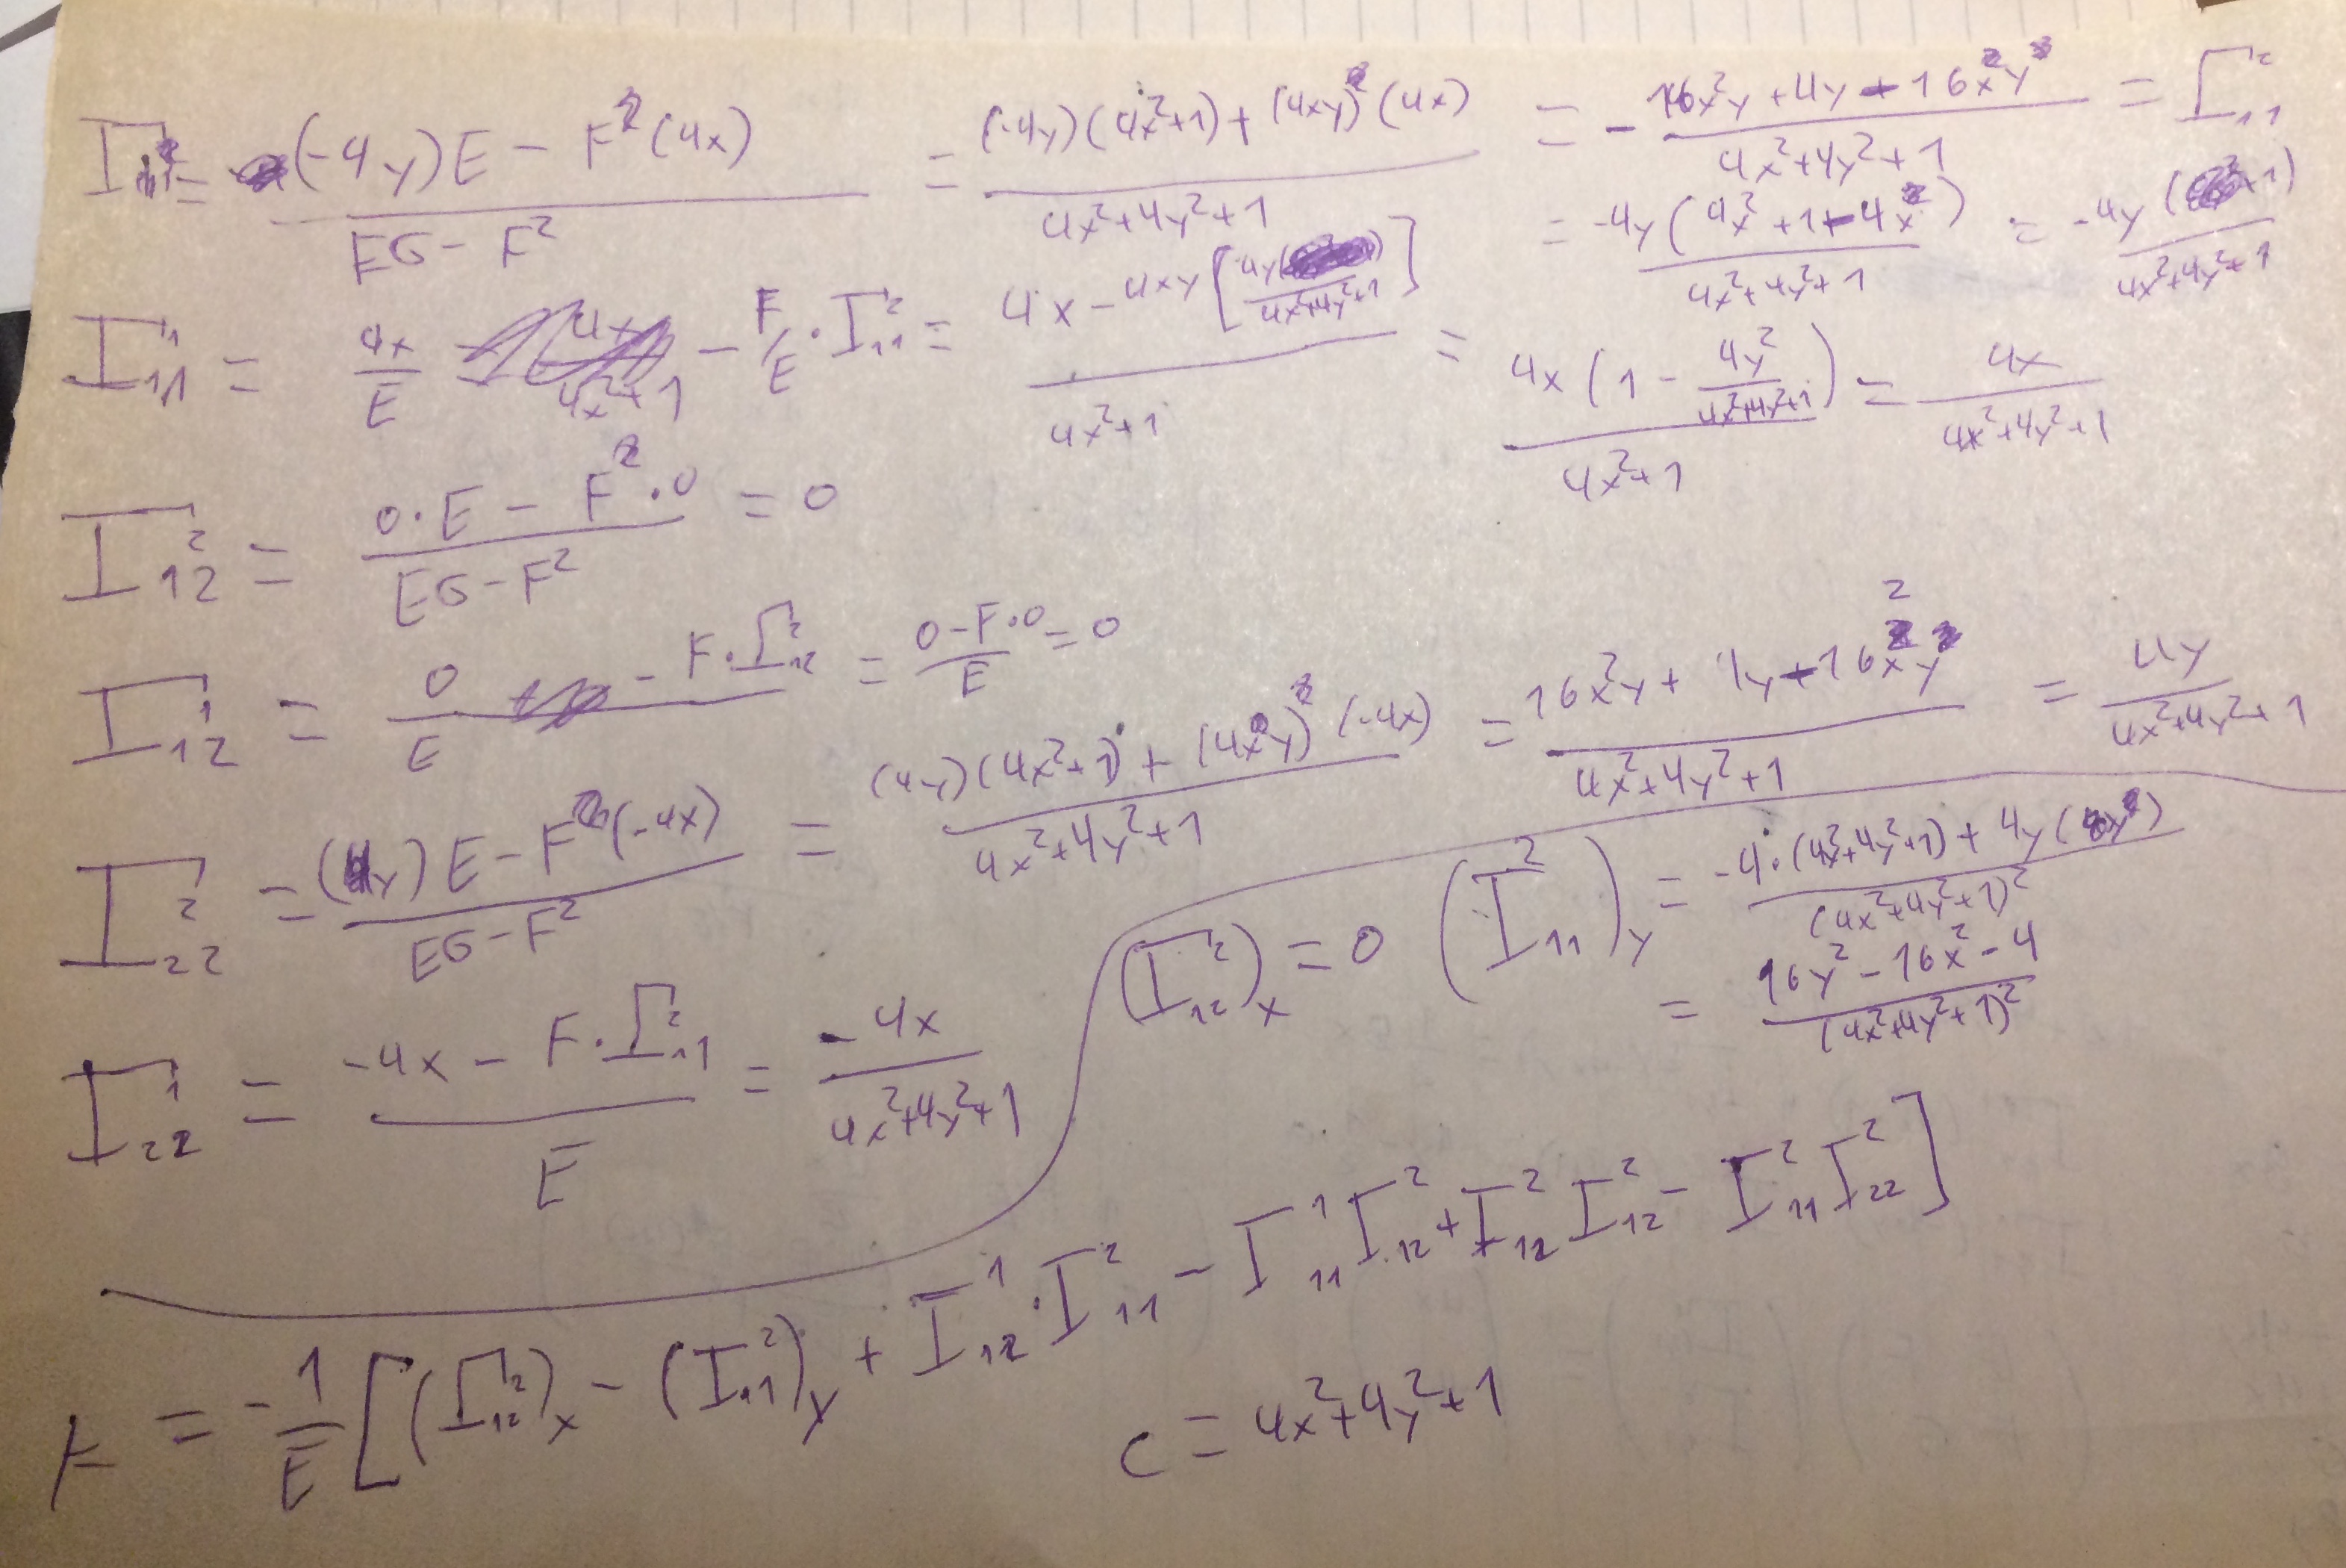
\includegraphics{img/IMG_5989.JPG}
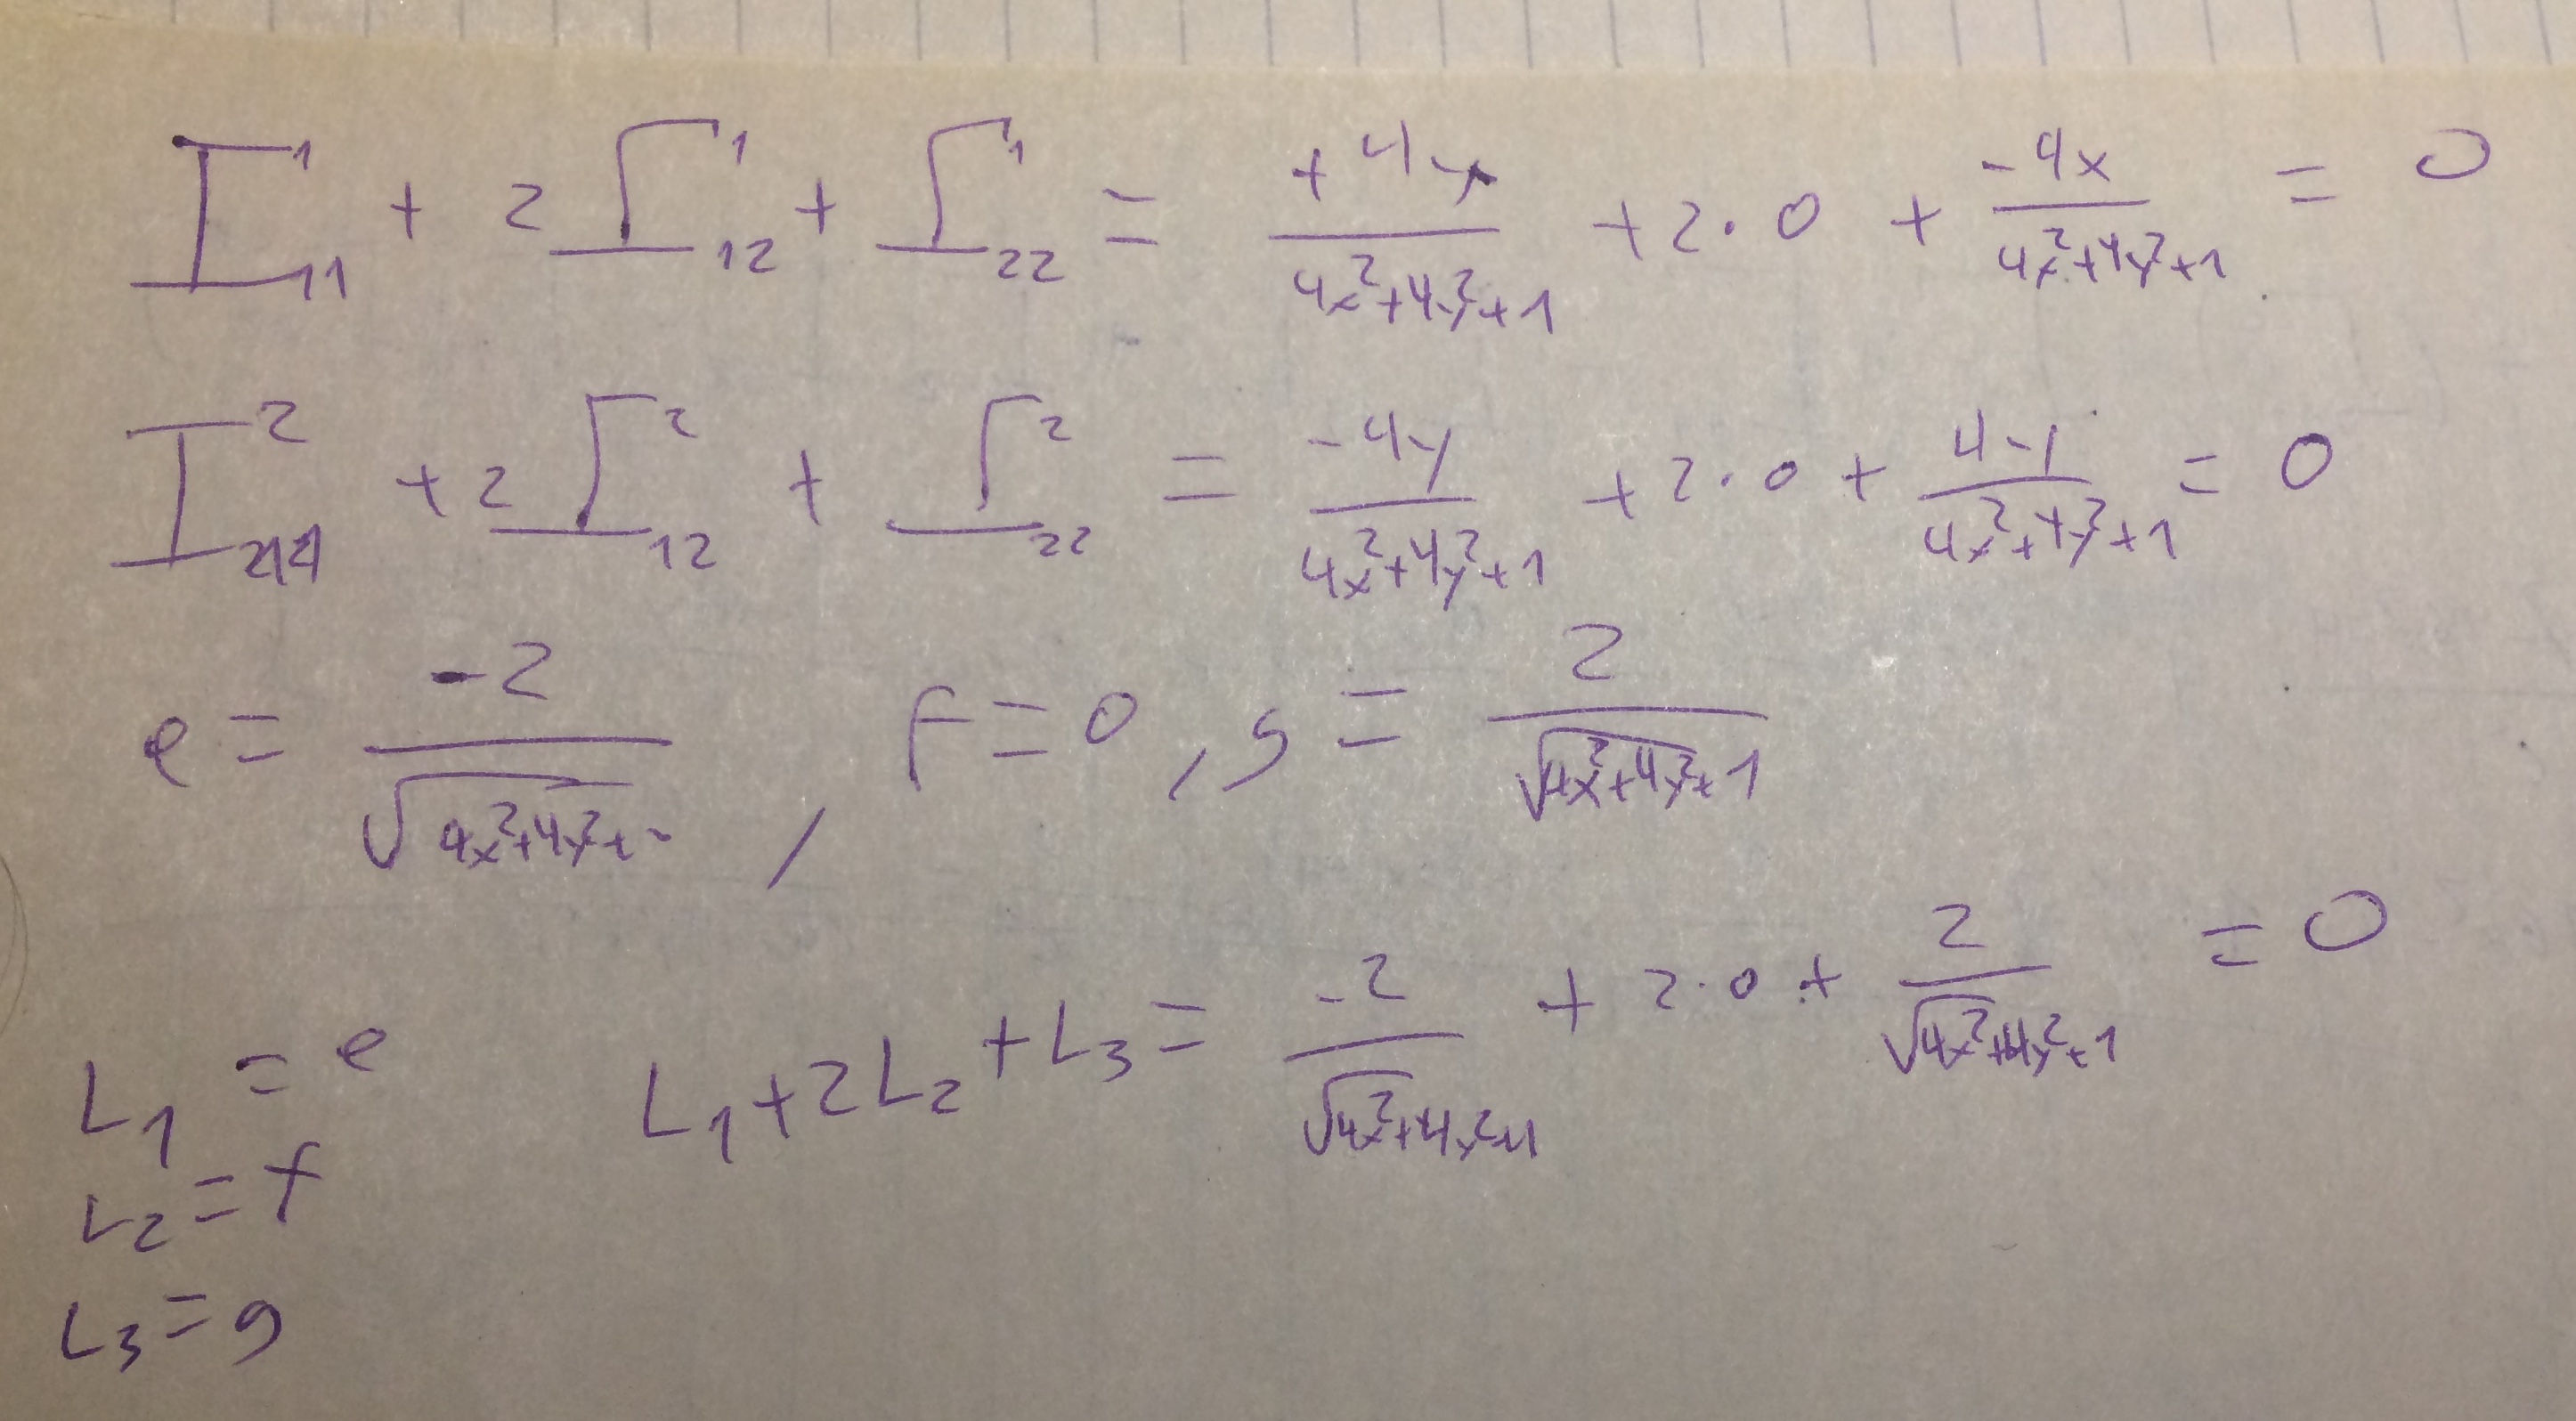
\includegraphics{img/IMG_5990.JPG}
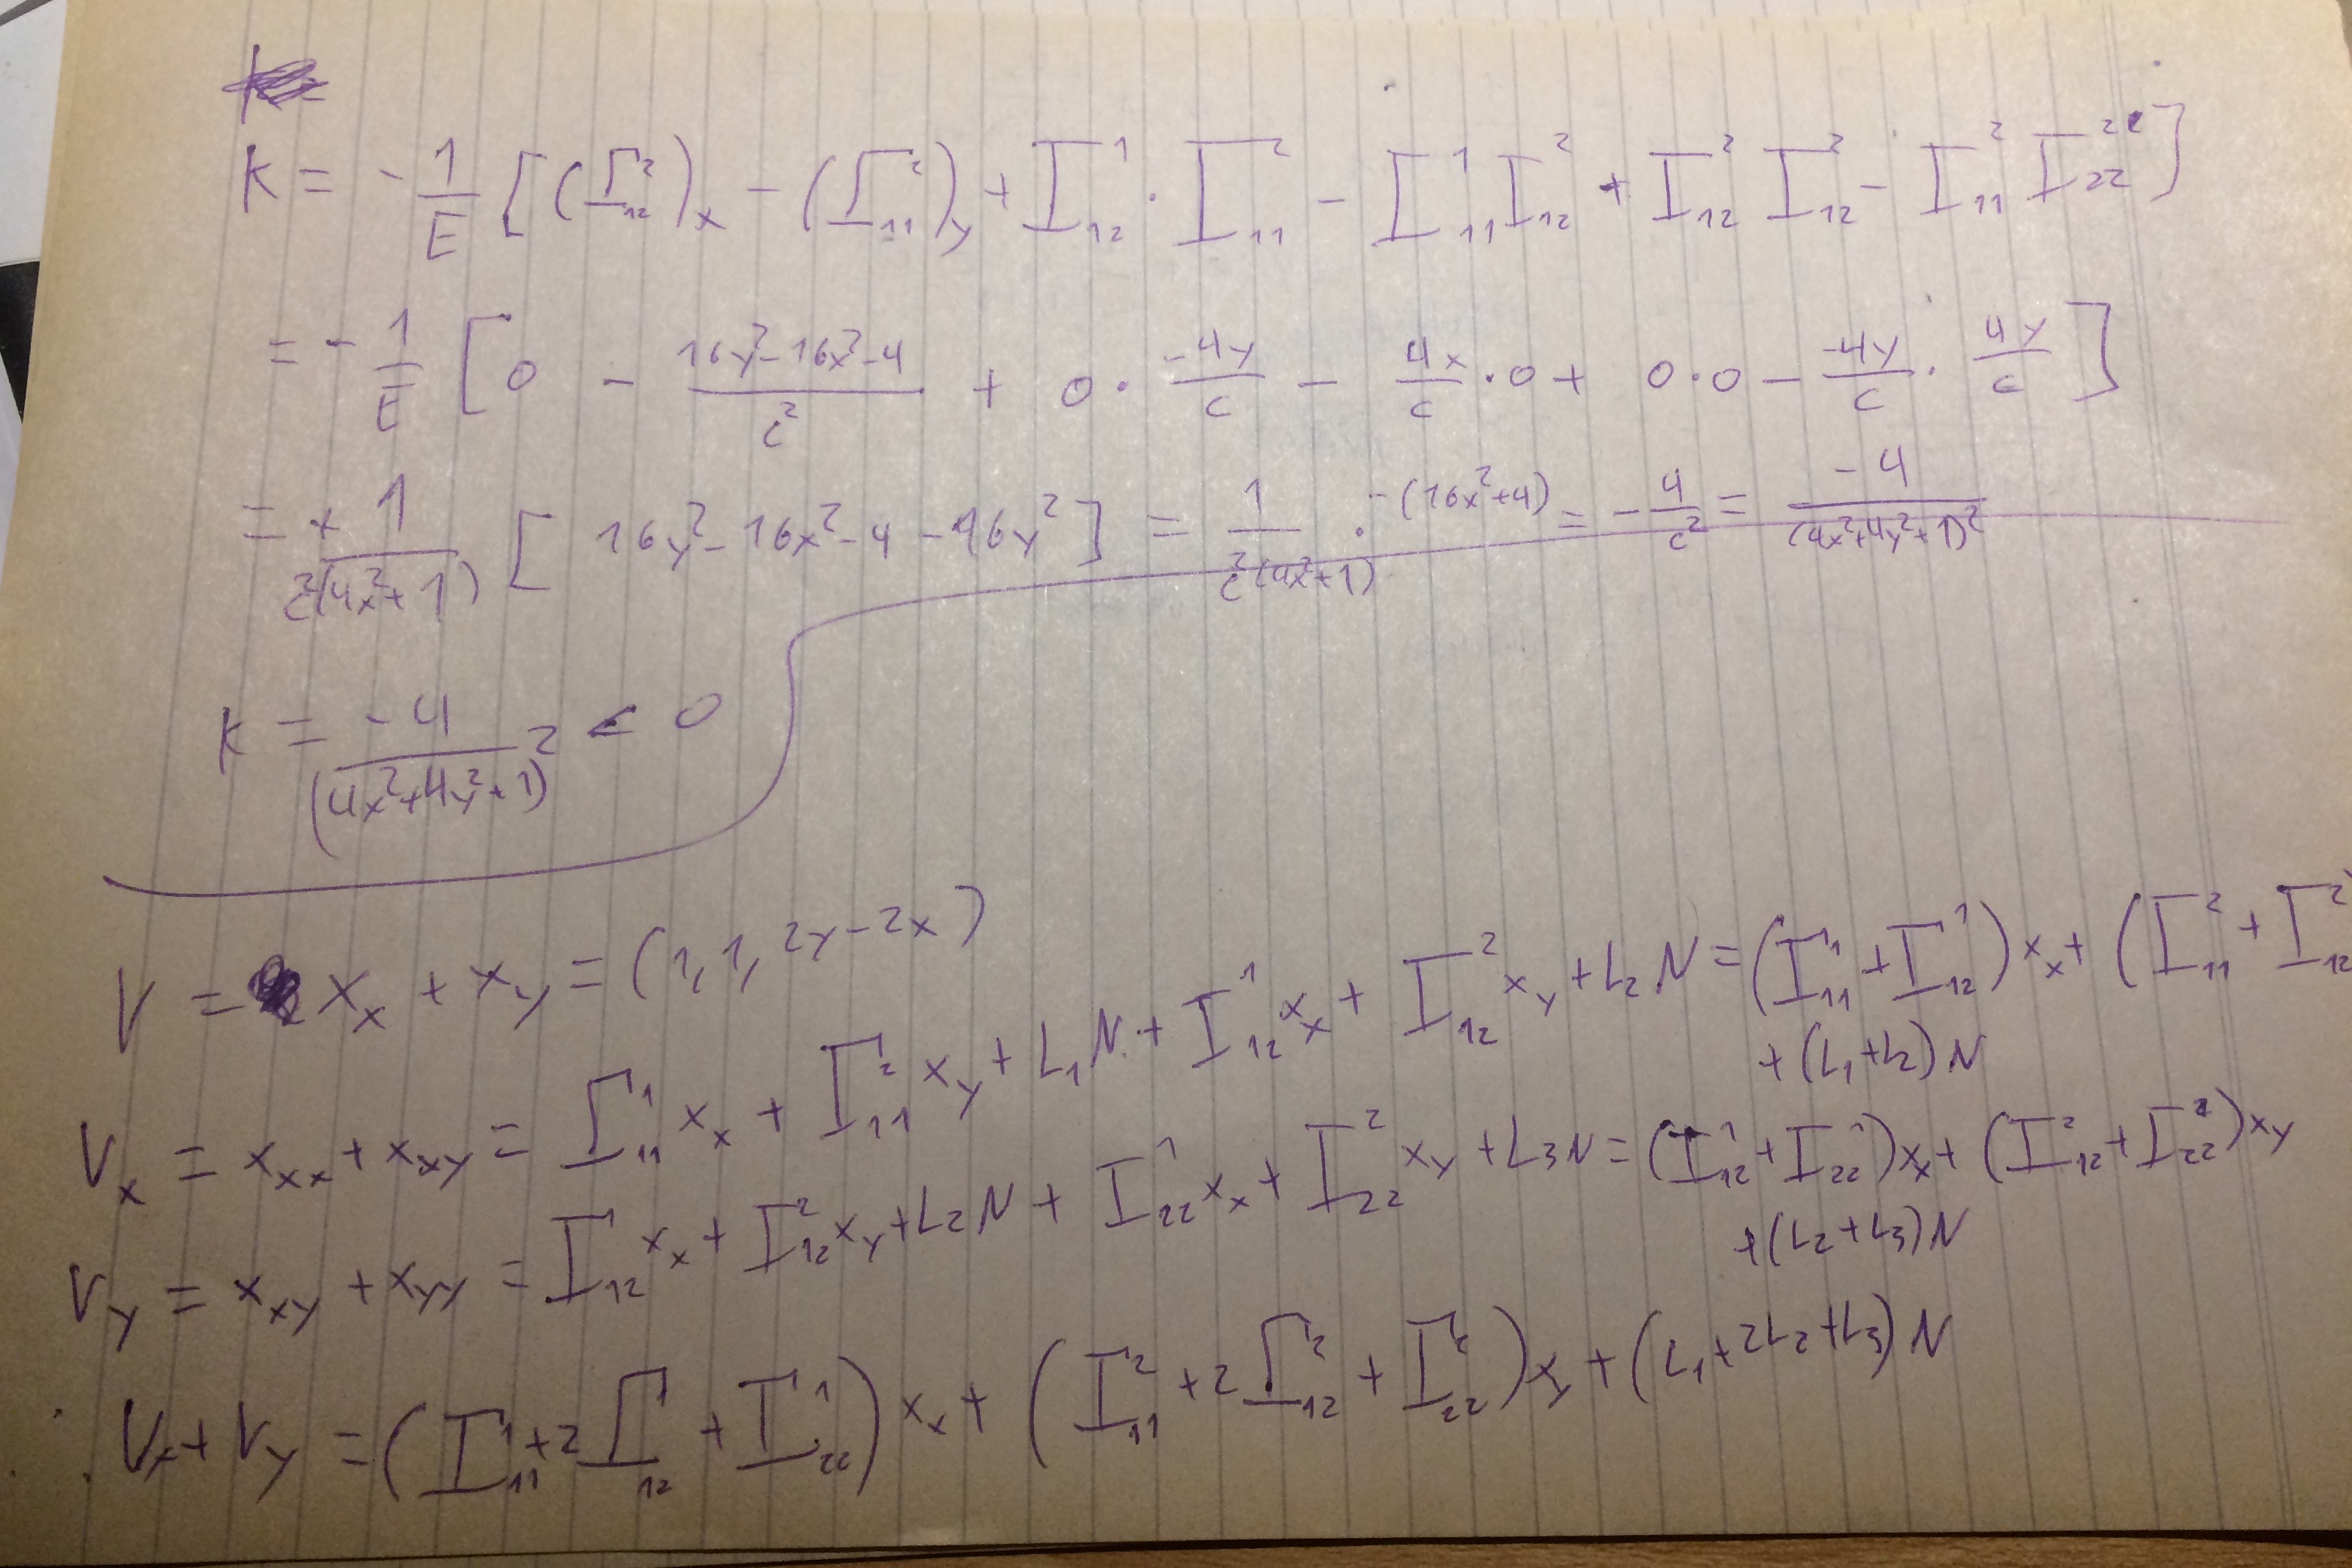
\includegraphics{img/IMG_5991.JPG}

\end{center}

\end{document}